% ============================================================
%  第二章  T=0 时费米系统的格林函数 —— 前半（§7–§13）
%  底本：印刷页 26–49（PDF 物理页 p036–p060）
%  章头 OCR 正文缺，按书前目录补（后半章 §14–§21 由 ch02b.tex 排入，不带 \chapter）。
%
%  插图清单：
%    图 1（p049，费米球面处分布函数的跃变）——占位 figures/fig1.pdf；
%      原书图无图注文字，仅"图 1"。原书图在正文右侧栏，此处排在"的极限值."
%      段之后（OCR 图块原在"于是我们有"句中，直接排入会割断行文）。
%    公式 (13.7)、(13.13)、(13.14) 为费曼图"图式"（编号公式）：
%      以清理后的 MinerU 裁剪位图排入（figures/feyn13-*.png），
%      放在 equation 环境中自动编号，恰为 (13.7)/(13.13)/(13.14)。
%      p056 ⟨S⟩ 分解小图（无编号）排为 equation*，figures/feyn13-loop.png。
%      如后续重绘矢量图可直接替换同名文件。
%
%  圈码脚注：共 21 处（①×18、②×3）已全部还原为 \footnote{...}（圈码字符
%  删除，圈码编号由 footmisc perpage 按页自动生成）。页面归属（PDF 页码，
%  以页面图核定）：p037①②、p038①、p039①、p040①、p041①（含两式）、
%  p043①、p044①②（②含主值积分式）、p046①、p047①、p051①、p052①、
%  p053①、p054①、p055①（含记号约定两式）、p056①、p057①、p058①②
%  （①含两式）、p060①。初稿所记 p036①②、p046 前移一页的 p045① 系页码
%  偏移，已按页面图纠正为 p037、p046。OCR 无脚注正文窜入段，无 %%FN 迁移项。
%
%  已修正的 OCR 错误（编号，注明依据页面）：
%   [1] p038 (7.2)：OCR 双层尖帽 \hat{\hat H'} → e^{iĤ't}（页面单帽）。
%   [2] p038 "(而不是给定 N 的那种 Ĥ)" → Ĥ'（页面带撇）。
%   [3] p039 (7.6) 第二个积分 OCR 小写 ψ̂ → Ψ̂（页面大写海森伯算符）。
%   [4] p039 (7.7) 第 4 行 ψ̂_α ψ̂_β → Ψ̂_α Ψ̂_β（页面大写）；V 的上标撇按页面保留。
%   [5] p039 (7.8) OCR "\dot A" → Δ（拉普拉斯算符）。
%   [6] p039 (7.9) ψ̂ → Ψ̂。
%   [7] p040 (7.13) OCR Ψ̂*_β → Ψ̂⁺_β（放大核对为加号）。
%   [8] p040 正文"令 F 为 F̂_αβ 某个'单粒子'算符"语序 → "令 F̂_αβ 为某个
%       '单粒子'算符"（页面）。
%   [9] p041 "乘积变成 Ψ̂_αΨ̂_α" → Ψ̂⁺_αΨ̂_α（页面有 +）。
%  [10] p042 (7.23) OCR 全乱（"d(−iωt/2π)·dω/t"）→ 按页面：
%       N(p) = −i lim_{t→−0} ∫ G(ω,p) e^{−iωt} dω/2π。
%  [11] p042 (8.1) 指数 ω_{nm^ℓ} → ω_{nm}t。
%  [12] p043 (8.4) 第 2 行 ψ̂ → Ψ̂⁺（页面大写带 +）；[13] 指数 ω_{mn}t 按页面
%       照排——按 (8.1) 应为 ω_{nm}，原书两处下标次序不一致，疑排印，登记待考。
%  [14] p043 "式中 ω_{0m}=E₀(N)−E_n(N+1)+μ" 的 E_n 按页面照排（按定义应为
%       E_m），疑原书排印，登记待考。
%  [15] p045 (8.13) 页面系数 4π⁴ 与 (8.7)/(8.12) 的 4π³ 不一致（δ 函数系数应
%       相同），疑原书排印错误，照排并登记。
%  [16] p045 准粒子色散律文献 OCR 乱（"[B. . - p,1955]"）→
%       [В. Л. Бонч-Бруевич, 1955]（页面俄文原名）。
%  [17] p047 跃变定义式 ψ̂ → Ψ̂（页面大写）。
%  [18] p048–49 (9.8)、(10.1)–(10.3) OCR ν_r → v_F。
%  [19] p050 "也有 𝔖 = 0" → "也有 S = 0"。
%  [20] p052 OCR "Ŝ(t₁−∞)" → Ŝ(t₁,−∞)（页面）。
%  [21] p053 "ŜΦ=⟨Ŝ⟩Φ. 恰好 Φ*Ŝ⁻¹=⟨S⟩Φ*" OCR 乱 → 按页面转写。
%  [22] p046–47 §9 首句 OCR 缺前半 → 按 p046 页面补"为了举例说明上一节所
%       讨论的普遍关系，我们来计算理想费米气体的"。
%  [23] p054 (13.3) 前 OCR 缺一句 → 按 p054 页面补"我们预先指出，按照维克
%       定理将公式(12.14)分子中的表达式展开时，例如"。
%  [24] p055 维克收缩四项展示 OCR 乱成 \neq 长串 → 按 p055 页面转写。原书
%       跨弧收缩无法用 amsmath 精确复刻，改用"端点标记法"：互相收缩的
%       一对算符加同种小弧标记（上弧 \frown、下弧 \smile、上浅弧 \smile）。
%  [25] p056 收缩代换式 OCR 乱 → ⌒Ψ₁Ψ₃⁺ ≡ ⟨TΨ̂₁Ψ̂₃⁺⟩ = iG⁰₁₃，
%       ⌒Ψ₂⁺Ψ₄ = −iG⁰₂₄，等等（"等等"二字 OCR 缺，按页面补）。
%  [26] p058 −G⁽⁰⁾_αγ(P)∫… 尾因子 OCR G^{(0)}_{αβ} → G^{(0)}_{δβ}（页面）。
%  [27] p059 k>1 圈图收缩式 OCR 乱 → 按页面 ⌒Ψ₁⁺Ψ₁ ⌒Ψ₂⁺Ψ₂ ⋯ ⌒Ψ_k⁺Ψ_k。
%  [28] p060 (13.15) â⁺ 上标 OCR "*" → +（页面）。
%  [29] p060 "只有成 ψ 对收缩" → "只有成对收缩"；"在极限 1/V, V→∞" →
%       "在极限 V→∞"（页面）。
%  [30] p041 (7.16) OCR "d^3 b x_1" → d³x₁。
%  [31] p036 章头缺 → 按书前目录补。
%
%  原书排印疑点（照排登记）：[12][13][14][15]；另 (7.7) 第 4 行
%  Ψ̂_α(t,r') 的 r' 与同行首因子宗量重复（按俄文原版疑应为另一宗量），
%  照原书页面排入，待考。
%
%  字体约定（对照页面核定）：化学势 μ 全章排粗体 \bm\mu（页面核对：
%  p044(8.7)、p044(8.10)、p048 正文、p050(11.1)(11.6) 均为粗体）；
%  激发能 ε 在 §8 排粗体（p044(8.9) 核对），§9–§10 的 ε(p) 排细体
%  （p048 正文核对），§11 (11.1) 的 ε 又为粗体（p050 核对），均照原书。
%  虚数单位排 \mathrm{i}。海森伯算符 Ψ̂ 用 \hat\Psi，薛定谔算符 ψ̂ 用 \hat\psi。
% ============================================================

\chapter{\texorpdfstring{$T=0$}{T=0} 时费米系统的格林函数}

\section{宏观系统的格林函数}

上一节所用的方法显得烦琐，在微扰论的高级近似中实际上已不再适用. 由于在实际的物理问题中，粒子之间的相互作用绝不是微弱的，因而这种方法的缺陷就更加突出. 于是，为了阐明宏观系统的各种普遍性质，需要研究微扰论级数的无穷项的集合. 有一种类似量子场论中所采用的数学技术可以克服这类困难.

这种数学工具的具体形式与需要运用它的宏观系统的性质有重要关系. 本章的以下几节，将阐述绝对零度时费米液体的数学工具的发展\footnote{В.\,М.\,Галицкий 和 А.\,Б.\,Мигдал（1958）系统地建立了这种数学工具.}. 在这里讲述的目的，不仅在于把方法实际应用到给定的客体上，而且也要表明这个工具大体是怎样建立的.

作为这个工具的原始资料，是二次量子化的 $\psi$ 算符，它们的性质在量子力学中已经讲过（见第三卷§64，§65）. 现在我们要用到作为时间显函数的海森伯绘景中的算符. 所以，将阐述这种绘景中 $\psi$ 算符的某些性质.

我们研究由自旋为1/2的粒子所构成的系统. 根据这种情况，应给 $\psi$ 算符加上表明自旋投影值的下标. 此下标取遍 $\pm 1/2$. 按以前的做法，我们将用希腊字母表示自旋下标，而列出两个重复下标表示求和.

根据一般规则（见第三卷§13），海森伯绘景中的任何物理量算符 $\hat f(t)$，都可以按照如下形式用（薛定谔绘景中）与时间无关的该物理量算符 $\hat f$ 表示出来\footnote{为了把公式写得简单，我们将广泛地采用量子常数 $\hbar=1$ 的单位制（因此动量具有 $\mathrm{cm}^{-1}$ 的量纲，而能量具有 $\mathrm{s}^{-1}$ 的量纲）. 要从这种单位制变到通常的单位制，公式中所有动量 $p$ 和能量 $E$ 都应代之以 $\bm p/\hbar$ 和 $E/\hbar$. 在这一章里就特别要采用这种单位.}：
\begin{equation*}
\hat f(t)=\mathrm{e}^{\mathrm{i}\hat Ht}\hat f\mathrm{e}^{-\mathrm{i}\hat Ht}
\end{equation*}
式中 $\hat H$ 为系统的哈密顿量.

但是，此处将对这个定义作些适当的修改. 因为，在不给定系统的粒子数 $N$ 而给定化学势 $\bm\mu$ 的情况，用量子统计学研究系统的状态比较方便. 这时，系统处于 $T=0$ 时的基态可定义为算符 $\hat H'$ 具有最小本征值的状态
\begin{equation}
\hat H'=\hat H-\bm\mu\hat N
\end{equation}
（而不是给定 $N$ 的那种 $\hat H'$）. 实际上，系统（当给定 $\bm\mu$ 值时）处于能量为 $E_n$ 和粒子数为 $N_n$ 的状态的概率是：
\begin{equation*}
w\propto\exp\bigg(-\frac{E_n-\mu N_n}{T}\bigg)=\exp\bigg(-\frac{E_n'}{T}\bigg)
\end{equation*}
［见第五卷(35.1)式］；这里 $E_n'$ 为算符 $\hat H'$ 的本征值，我们看到，当 $T=0$ 时，只是 $E_n'$ 为最小值的状态\footnote{如同 $\hat H$ 一样，我们将称算符 $\hat H'$ 为哈密顿量.}.

所以，可用公式
\begin{equation}
\begin{aligned}
\hat\Psi_\alpha(t,\bm r)&=\mathrm{e}^{\mathrm{i}\hat H't}\hat\psi_\alpha(\bm r)\mathrm{e}^{-\mathrm{i}\hat H't},\\
\hat\Psi^{+}_\alpha(t,\bm r)&=\mathrm{e}^{\mathrm{i}\hat H't}\hat\psi^{+}_\alpha(\bm r)\mathrm{e}^{-\mathrm{i}\hat H't}
\end{aligned}
\end{equation}
来定义海森伯绘景中的 $\psi$ 算符. 我们将用大写字母 $\hat\Psi$ 来表征海森伯绘景中的 $\psi$ 算符，而用小写字母 $\hat\psi$ 表征薛定谔绘景中的 $\psi$ 算符.

薛定谔绘景中的 $\psi$ 算符满足熟知的对易规则. 而对于取不同时刻 $t$ 和 $t'$ 的海森伯算符的对易子，却不能以普遍形式算出来. 但是当 $t=t'$ 时，海森伯算符的对易规则与薛定谔算符的对易规则是相同的. 例如，根据规则
\begin{equation*}
\hat\psi_\alpha(\bm r)\hat\psi^{+}_\beta(\bm r')+\hat\psi^{+}_\beta(\bm r')\hat\psi_\alpha(\bm r)=\delta_{\alpha\beta}\delta(\bm r-\bm r'),
\end{equation*}
可以得到类似的规则：
\begin{equation}
\begin{aligned}
&\hat\Psi_\alpha(t,\bm r)\hat\Psi^{+}_\beta(t,\bm r')+\hat\Psi^{+}_\beta(t,\bm r')\hat\Psi_\alpha(t,\bm r)=\\
&=\mathrm{e}^{\mathrm{i}\hat H't}\big(\hat\psi_\alpha(\bm r)\hat\psi^{+}_\beta(\bm r')+\hat\psi^{+}_\beta(\bm r')\hat\psi_\alpha(\bm r)\big)\mathrm{e}^{-\mathrm{i}\hat H't}=\\
&=\delta_{\alpha\beta}\delta(\bm r-\bm r'),
\end{aligned}
\end{equation}
所以：
\begin{equation}
\begin{aligned}
&\hat\Psi_\alpha(t,\bm r)\hat\Psi_\beta(t,\bm r')+\hat\Psi_\beta(t,\bm r')\hat\Psi_\alpha(t,\bm r)=0,\\
&\hat\Psi^{+}_\alpha(t,\bm r')\hat\Psi^{+}_\beta(t,\bm r')+\hat\Psi^{+}_\beta(t,\bm r')\hat\Psi^{+}_\alpha(t,\bm r')=0,
\end{aligned}
\end{equation}

将定义式(7.2)对时间取微商，我们求得海森伯算符满足的方程：
\begin{equation}
-\mathrm{i}\,\frac{\partial}{\partial t}\hat\Psi_\alpha(t,\bm r)=\hat H'\hat\Psi_\alpha(t,\bm r)-\hat\Psi_\alpha(t,\bm r)\hat H'
\end{equation}
［见第三卷(13.7)式］.

对于任何守恒量算符（即同哈密顿量可对易的算符），海森伯绘景和薛定谔绘景是等同的. 例如，哈密顿量本身、粒子数算符（当然粒子数也是守恒量）都是这类算符. 这些算符用薛定谔算符或用海森伯算符表达都一样. 于是，粒子数算符
\begin{equation}
\hat N=\int\hat\psi^{+}_\alpha(\bm r)\hat\psi_\alpha(\bm r)\,\mathrm{d}^3x=\int\hat\Psi^{+}_\alpha(t,\bm r)\hat\Psi_\alpha(t,\bm r)\,\mathrm{d}^3x.
\end{equation}

相互作用粒子系统的哈密顿量为
\begin{equation}
\begin{aligned}
&\hat H'=\hat H'^{(0)}+\hat V'^{(1)}+\hat V'^{(2)}+\cdots,\\
&\hat H'^{(0)}=-\frac{1}{2m}\int\hat\Psi^{+}_\alpha(t,\bm r)\Delta\hat\Psi_\alpha(t,\bm r)\,\mathrm{d}^3x-\mu\hat N,\\
&\hat V'^{(1)}=\int\hat\Psi^{+}_\alpha(t,\bm r)U^{(1)}(\bm r)\hat\Psi_\alpha(t,\bm r)\,\mathrm{d}^3x,\\
&\hat V'^{(2)}=\frac{1}{2}\int\hat\Psi^{+}_\beta(t,\bm r')\hat\Psi^{+}_\alpha(t,\bm r')U^{(2)}(\bm r-\bm r')\hat\Psi_\alpha(t,\bm r')\hat\Psi_\beta(t,\bm r)\,\mathrm{d}^3x\,\mathrm{d}^3x'.
\end{aligned}
\end{equation}

这里 $\hat H'^{(0)}$ 为自由粒子系统的哈密顿量；$\hat V'^{(1)}$ 为自由粒子与外场 $U^{(1)}(\bm r)$ 相互作用算符；$\hat V'^{(2)}$ 是粒子对的相互作用算符，其中 $U^{(2)}(\bm r-\bm r')$ 是两个粒子的相互作用能；省略的各项是三重及三重以上的相互作用［见第三卷(64.25)式］. 为简单起见，假定所有的相互作用都与粒子的自旋无关.

(7.5)式中 $\hat H'$ 与 $\hat\Psi_\alpha$ 的对易子，可以用规则(7.3—7.4)算出；其间出现的 $\delta$ 函数被积分消除了. 结果得到了如下形式的关于 $\hat\Psi_\alpha(t,\bm r)$ 的“薛定谔方程”：
\begin{equation}
\begin{aligned}
\mathrm{i}\frac{\partial}{\partial t}\hat\Psi_\alpha(t,\bm r)&=\Big(-\frac{1}{2m}\Delta-\mu+U^{(1)}(\bm r)\Big)\hat\Psi_\alpha(t,\bm r)+\\
&+\int\hat\Psi^{+}_\beta(t,\bm r')U^{(2)}(\bm r-\bm r')\hat\Psi_\beta(t,\bm r')\,\mathrm{d}^3x'\cdot\hat\Psi_\alpha(t,\bm r)+\cdots.
\end{aligned}
\end{equation}

在所讲述的方法中，宏观系统的格林函数概念起着基本作用. 它由下式定义\footnote{这个定义类似于量子电动力学中精确的格林函数（传播子）的定义（见第四卷 §103，§105）.}：
\begin{equation}
G_{\alpha\beta}(X_1,X_2)=-\mathrm{i}\langle T\hat\Psi_\alpha(X_1)\hat\Psi^{+}_\beta(X_2)\rangle.
\end{equation}

为简略起见，今后用 $X$ 表征时刻 $t$ 和点的径矢 $\bm r$ 的总体. 角括号$\langle\cdots\rangle$表征按系统基态的平均值（代替较烦琐的对角矩阵元记号 $\langle0|\cdots|0\rangle$）. 记号 $T$ 是编时乘积的标志：$T$ 后的算符应按时间 $t_1,t_2$ 增长的次序从右向左排列. 同时，在费米子的情况下，置换一对 $\psi$ 算符应随之改变乘积的符号（与原先书写乘积时的排列相比较）. 用显形式表达，即为
\begin{equation}
G_{\alpha\beta}(X_1,X_2)=
\begin{cases}
-\mathrm{i}\langle\hat\Psi_\alpha(X_1)\hat\Psi^{*}_\beta(X_2)\rangle,& t_1>t_2;\\
\mathrm{i}\langle\hat\Psi^{*}_\beta(X_2)\hat\Psi_\alpha(X_1)\rangle,& t_1<t_2.
\end{cases}
\end{equation}

现在我们来指出格林函数某些明显的性质. 如果系统不是铁磁的，也不处于外场中，则格林函数的自旋关系归结为单位矩阵：
\begin{equation}
G_{\alpha\beta}(X_1,X_2)=\delta_{\alpha\beta}G(X_1,X_2)
\end{equation}
（任何其他形式的依赖关系均需标出空间中的选定方向——自旋量子化的 $z$ 轴）\footnote{这个说法需要解释. 自旋分量 $\hat\Psi_{\alpha}$ 是一阶逆变旋量（在这个意义上说，若采用带有上标 $\alpha$ 的记号 $\hat\Psi^{\alpha}$ 更为合适），而分量 $\hat\Psi^{+}_{\beta}$ 是协变旋量. 所以 $G_{\alpha\beta}$ 是二阶混合旋量. 二阶单位混合旋量就是 $\delta_{\alpha\beta}$.}. 由于时间的均匀性，时刻 $t_1$ 和 $t_2$ 仅以差的形式 $t=t_1-t_2$ 出现在格林函数中. 此外，如果宏观系统在空间是均匀的，那么两点的坐标也仅以差的形式 $\bm r=\bm r_1-\bm r_2$ 出现在格林函数中. 换言之，在这种情况下
\begin{equation}
G_{\alpha\beta}(X_1,X_2)=\delta_{\alpha\beta}G(X),\qquad X=X_1-X_2.
\end{equation}

我们强调一下，微观均匀性的意思是：假定物体不仅本身的（宏观）平均密度是均匀的，而且物体的粒子在空间不同的（微观）位置的概率密度也是均匀的. 这种物体正是液体和气体（但不是固态晶体）. 由于它们是各向同性的，所以 $G(t,\bm r)=G(t,-\bm r)$. 说到这里我们再一次强调，这时函数 $G(t,\bm r)$，按其本身的定义绝不是 $t$ 的偶函数. 就这个意义上说，$t_1$ 和 $t_2$ 在差 $t=t_1-t_2$ 中的次序是很重要的.

系统中粒子坐标的密度矩阵，定义为平均值：
\begin{equation}
\rho_{\alpha\beta}(\bm r_1,\bm r_2)=\frac{1}{N}\big\langle\hat\Psi^{+}_\beta(t,\bm r_2)\hat\Psi_\alpha(t,\bm r_1)\big\rangle.
\end{equation}

知道了这个矩阵，就能求出关于单个粒子的任何量的平均值. 实际上，令 $\hat F_{\alpha\beta}$ 为某个“单粒子”算符，即形为
\begin{equation}
\hat F_{\alpha\beta}=\sum_a\hat f^{(a)}_{\alpha\beta}
\end{equation}
的算符，式中 $\hat f^{(a)}_{\alpha\beta}$ 是只作用在一个（第 $a$ 个）粒子的坐标和自旋的算符，而求和是遍及系统的全部粒子. 用二次量子化的工具可以把这个算符（在海森伯绘景中）写成
\begin{equation}
\hat F_{\alpha\beta}(t)=\int\hat\Psi^{+}_\alpha(t,\bm r)\hat f_{\beta\gamma}\hat\Psi_\gamma(t,\bm r)\,\mathrm{d}^3x
\end{equation}
［见第三卷(64.23)式］. 由此可见，$F$ 的平均值可用密度矩阵的术语表示成如下形式：
\begin{equation}
\langle F\rangle=N\langle f\rangle=N\int\big[\hat f^{(1)}_{\alpha\beta}\rho_{\beta\alpha}(\bm r_1,\bm r_2)\big]_{r_2=r_1}\,\mathrm{d}^3x_1
\end{equation}
式中 $\hat f^{(1)}_{\alpha\beta}$ 为作用在坐标 $\bm r_1$ 的算符（应当在算符作用之后，而在积分之前取 $\bm r_2=\bm r_1$）.

根据(7.10)式，密度矩阵可用格林函数表达为
\begin{equation}
\rho_{\alpha\beta}(\bm r_1,\bm r_2)=-\frac{\mathrm{i}}{N}G_{\alpha\beta}(t_1,\bm r_1;t_1+0,\bm r_2).
\end{equation}

今后凡取 $t_1+0$ 形的函数宗量记号，均指宗量有从大于方面趋于 $t_1$ 值的极限. 取这个极限可以保证 $\psi$ 算符的正确次序，它与(7.13)式乘积中算符的次序相同.

对于微观均匀系统，密度矩阵只依赖于差 $\bm r=\bm r_1-\bm r_2$，当与自旋无关时，$\rho_{\alpha\beta}=\delta_{\alpha\beta}\rho$，并且
\begin{equation}
\rho(\bm r)=-\frac{\mathrm{i}}{N}G(t=-0,\bm r).
\end{equation}

这里，根据(7.12)式，引用函数 $G(X_1-X_2)\equiv G(X)$ 代替 $G_{\alpha\beta}(X_1,X_2)$. 当 $\bm r_1=\bm r_2$ 时，并按自旋变量取迹之后，(7.13)式中的算符的乘积变成 $\hat\Psi^{+}_\alpha\hat\Psi_\alpha$（系统中粒子数密度算符）. 所以，物体的平均密度
\begin{equation}
\frac{N}{V}=2N\rho(0)=-2\mathrm{i}G(t=-0,\bm r=0)
\end{equation}
（$t$ 从小于方面趋于零）. 这个等式把 $T=0$ 时的化学势 $\mu$（$G$ 同 $\bm\mu$ 的关系是将后者作为参量）与粒子数密度 $N/V$ 联系起来了.

函数 $\rho(\bm r_1,\bm r_2)$ 的傅里叶展开，确定了粒子按动量的分布\footnote{我们提醒一下，（见第三卷 §14），单粒子的密度矩阵是如下的积分：
\begin{equation*}
\rho(\bm r_{1},\bm r_{2})=\int\Psi^{*}(\bm r_{2},q)\,\Psi(\bm r_{1},q)\,\mathrm{d}q,
\end{equation*}
式中 $\Psi(\bm r,q)$ 为整个系统的波函数，其中 $\bm r$ 表示一个粒子的径矢，而 $q$ 为其余所有粒子的坐标的总合，因此是对 $q$ 积分. 密度矩阵的傅里叶分量与下式相同：
\begin{equation*}
\int\Bigl|\int\Psi(\bm r,q)\,\mathrm{e}^{\mathrm{i}\bm p\cdot\bm r}\,\mathrm{d}^{3}x\Bigr|^{2}\,\mathrm{d}q,
\end{equation*}
因而得到密度矩阵与粒子按动量分布的关系.}
\begin{equation}
\begin{aligned}
N(\bm p)&=N\int\rho(\bm r_1,\bm r_2)\mathrm{e}^{-\mathrm{i}\bm p\cdot(\bm r_1-\bm r_2)}\,\mathrm{d}^3(\bm x_1-\bm x_2)=\\
&=-\mathrm{i}\int G(t,\bm r)\big|_{t=-0}\,\mathrm{e}^{-\mathrm{i}\bm p\cdot\bm r}\,\mathrm{d}^3x.
\end{aligned}
\end{equation}

这就是单位体积内具有一定的自旋投影值并且动量在 $\mathrm{d}^3p/(2\pi)^3$ 区间内的粒子数. 我们强调，这里所说的是真实粒子，而不是准粒子（后者在所讲述的工具中还没有出现！）。这里引用记号 $N(\bm p)$ 以区别于准粒子的分布函数 $n(\bm p)$.

今后，我们通常要和动量表象中的格林函数打交道，它定义为函数 $G(t,\bm r)$ 按 $t$ 和 $\bm r$ 的傅里叶展开的分量：
\begin{equation}
G(t,\bm r)=\int G(\omega,\bm p)\,\mathrm{e}^{\mathrm{i}(\bm p\cdot\bm r-\omega t)}\frac{\mathrm{d}\omega\,\mathrm{d}^3p}{(2\pi)^4},
\end{equation}
\begin{equation}
G(\omega,\bm p)=\int G(t,\bm r)\,\mathrm{e}^{-\mathrm{i}(\bm p\cdot\bm r-\omega t)}\mathrm{d}t\,\mathrm{d}^3x.
\end{equation}

粒子按动量的分布，是通过这个函数并由公式
\begin{equation}
N(\bm p)=-\mathrm{i}\lim_{t\to-0}\int_{-\infty}^{\infty}G(\omega,\bm p)\,\mathrm{e}^{-\mathrm{i}\omega t}\frac{\mathrm{d}\omega}{2\pi}
\end{equation}
表达. 这个公式是将(7.21)式代入(7.20)式得到的. 它的归一化表成公式：
\begin{equation}
-2\mathrm{i}\lim_{t\to-0}\int G(\omega,\bm p)\,\mathrm{e}^{-\mathrm{i}\omega t}\frac{\mathrm{d}\omega\,\mathrm{d}^3p}{(2\pi)^4}=\frac{N}{V},
\end{equation}
这就是在动量表象表述的条件(7.19). 因此，分布 $N(\bm p)$ 自然正确地归一为：
\begin{equation*}
2\int N(\bm p)\frac{\mathrm{d}^3p}{(2\pi)^3}=\frac{N}{V}.
\end{equation*}

我们指出，(7.23—7.24)式的积分所取的极限等价于复变量 $\omega$ 平面内的一定绕行规则. 因为有 $t<0$ 的因子 $\mathrm{e}^{-\mathrm{i}\omega t}$ 存在，便能用 $\bm\omega$ 上半平面内无限远的半圆周来封闭积分路线（实轴），于是积分便由函数 $G(\omega,\bm p)$ 在这个半平面内的诸极点的留数所决定.

\section{依格林函数确定能谱}

就微观均匀系统来说，对于具有一定能量和动量值的定态，容易求出海森伯 $\psi$ 算符的矩阵元与时间和坐标的关系.

我们用通常的指数因子给出与时间的关系：
\begin{equation}
\langle n|\hat\Psi_\alpha(t,\bm r)|m\rangle=\mathrm{e}^{\mathrm{i}\omega_{nm}t}\langle n|\hat\psi_\alpha(\bm r)|m\rangle.
\end{equation}

但是，由于海森伯 $\psi$ 算符是利用哈密顿量 $\hat H'$ 定义的，所以
\begin{equation*}
\omega_{nm}=E_n'-E_m'=E_n-E_m-\mu(N_n-N_m).
\end{equation*}

根据 $\psi$ 算符的一般性质，算符 $\hat\Psi$ 使系统中的粒子数减少1（而 $\hat\Psi^{+}$ 使粒子数增加1）. 所以，在矩阵元(8.1)中 $N_n=N_m-1$，因此，
\begin{equation}
\omega_{nm}=E_n(N)-E_m(N+1)+\mu,
\end{equation}
这里，处于相应态中的粒子数是以宗量形式表示的.

为了求出对坐标的依赖关系，我们指出：由于系统的均匀性，当相对于系统移动任一距离 $\bm r$ 时，它的 $\psi$ 算符的矩阵元不会改变. 但是，这并不意味矩阵元根本与坐标无关. 因为 $\psi_{nm}(\bm r)$ 与在一个给定的 $\bm r=0$ 点的值 $\psi_{nm}(\bm 0)$ 的区别涉及两个原因：一是与相对于系统本身移动的距离 $\bm r$ 有关；其次与观察点向空间另一处的位移有关，这时也改变波函数的相位. 为了消除波函数位相的这个变化，我们把系统移动一矢量 $-\bm r$，也就是把平移算符
\begin{equation*}
\hat T(-\bm r)=\mathrm{e}^{-\mathrm{i}\bm r\cdot\hat{\bm P}}
\end{equation*}
作用到系统的波函数上［式中 $\hat{\bm P}$ 为系统的总动量算符；见第三卷(15.13)式］. 经这些运算之后，观察点又回到起始的空间位置，但仍然相对于系统移动了矢量 $\bm r$. 矩阵元对于这种变换的不变性，可用下列等式表达：
\begin{equation}
\langle n|\hat\psi_\alpha(\bm 0)|m\rangle=\big\langle n\big|\mathrm{e}^{\mathrm{i}\bm r\cdot\hat{\bm P}}\hat\psi_\alpha(\bm r)\mathrm{e}^{-\mathrm{i}\bm r\cdot\hat{\bm P}}\big|m\big\rangle.
\end{equation}

如果系统处于 $n$ 和 $m$ 态上具有确定的动量 $\bm P_n$ 和 $\bm P_m$，那么
\begin{equation*}
\langle n|\hat\psi_\alpha(\bm 0)|m\rangle=\mathrm{e}^{\mathrm{i}\bm k_{nm}\cdot\bm r}\langle n|\hat\psi_\alpha(\bm r)|m\rangle,
\end{equation*}
因而，
\begin{equation}
\begin{aligned}
\langle n|\hat\Psi_\alpha(t,\bm r)|m\rangle&=\mathrm{e}^{\mathrm{i}(\omega_{mn}t-\bm k_{nm}\cdot\bm r)}\langle n|\hat\psi_\alpha(\bm 0)|m\rangle,\\
\langle n|\hat\Psi^{+}_\alpha(t,\bm r)|m\rangle&=\langle m|\hat\Psi_\alpha(t,\bm r)|n\rangle^{*},
\end{aligned}
\end{equation}
式中 $\bm k_{nm}=\bm P_n-\bm P_m$.

用这些公式可以得到格林函数在动量空间的重要展开式，它使格林函数的物理意义更明显了.

由于函数 $G(t,\bm r)$ 的“不连续”定义，在计算 $G(\omega,\bm p)$ 时应把(7.22)式中对 $\mathrm{d}t$ 的积分分为由 $-\infty$ 到0和由0到 $\infty$ 两个积分. 在第二个积分里（即 $t=t_1-t_2>0$ 时），根据矩阵乘法规则将定义(7.10)展开，我们有：
\begin{equation*}
G(t,\bm r)=\frac{1}{2}G_{\alpha\alpha}=-\frac{\mathrm{i}}{2}\sum_m\langle0|\hat\Psi_\alpha(X_1)|m\rangle\langle m|\hat\Psi^{+}_\alpha(X_2)|0\rangle
\end{equation*}
（按系统的全部量子态求和）. 将(8.4)式代入此式，并注意到在基态时 $\bm P_0=\bm 0$，我们求得：
\begin{equation}
G(t,\bm r)=-\frac{\mathrm{i}}{2}\sum_m\big|\langle0|\hat\psi_\alpha(\bm 0)|m\rangle\big|^2\mathrm{e}^{\mathrm{i}(\omega_{0m}t+\bm P_m\cdot\bm r)},
\end{equation}
式中 $\omega_{0m}=E_0(N)-E_n(N+1)+\bm\mu$.

在(7.22)式中［其中 $G(t,\bm r)$ 由(8.5)式确定］对空间取积分，可以在求和式的每一项中得到 $\delta$ 函数 $\delta(\bm p-\bm P_m)$. 而对 $\mathrm{d}t$ ($t>0$) 积分时，为了保证收敛，需给 $\omega$ 增添一个无限小的正虚部，即以 $\omega+\mathrm{i}0$ 代替 $\omega$\footnote{这种手续类似于量子电动力学中计算格林函数的方法（对照第四卷 §75）.}. 于是得到：
\begin{equation*}
\iint_0^{\infty}G(t,\bm r)\,\mathrm{e}^{\mathrm{i}(\omega t-\bm p\cdot\bm r)}\,\mathrm{d}^3x\,\mathrm{d}t=\frac{(2\pi)^3}{2}\sum_m\big|\langle0|\hat\psi_\alpha(\bm 0)|m\rangle\big|^2\frac{\delta(\bm p-\bm P_m)}{\omega+\omega_{0m}+\mathrm{i}0}.
\end{equation*}

同样，可以算出对 $\mathrm{d}t$ 由 $-\infty$ 到0的积分. 当 $t<0$ 时，代替(8.5)式，有
\begin{equation}
G(t,\bm r)=\frac{\mathrm{i}}{2}\sum_m\big|\langle m|\hat\psi_\alpha(\bm 0)|0\rangle\big|^2\mathrm{e}^{\mathrm{i}(\omega_{m0}t-\bm P_m\cdot\bm r)},
\end{equation}
式中 $\omega_{m0}=E_m(N-1)-E_0(N)+\bm\mu$. 现在算出由 $-\infty$ 到0的积分，并将两个积分加在一起，可得：
\begin{equation}
\begin{aligned}
G(\omega,\bm p)=\frac{(2\pi)^3}{2}\sum_m\Big\{&\frac{A_m\delta(\bm p-\bm P_m)}{\omega+\bm\mu+E_0(N)-E_m(N+1)+\mathrm{i}0}+\\
&+\frac{B_m\delta(\bm p+\bm P_m)}{\omega+\bm\mu+E_m(N-1)-E_0(N)-\mathrm{i}0}\Big\},
\end{aligned}
\end{equation}
式中的记号
\begin{equation}
A_m=\big|\langle0|\hat\psi_\alpha(\bm 0)|m\rangle\big|^2,\quad B_m=\big|\langle m|\hat\psi_\alpha(\bm 0)|0\rangle\big|^2.
\end{equation}

这就是所求的展开式\footnote{量子场论中类似的展开式，称为 K\"all\'en--Lehmann 公式（对照第四卷 §104，§111）.}.

我们引入激发能的记号：
\begin{equation}
\bm\varepsilon^{(+)}_m=E_m(N+1)-E_0(N),\qquad \bm\varepsilon^{(-)}_m=E_0(N)-E_m(N-1).
\end{equation}

它们由一定粒子数的系统的激发能级与多一个或少一个粒子系统的基态能级之差来确定. 上标 $(+)$ 和 $(-)$ 表示这些能量：
\begin{equation}
\bm\varepsilon^{(+)}_m>\bm\mu,\qquad \bm\varepsilon^{(-)}_m<\bm\mu.
\end{equation}

实际上，只要注意到 $E_0(N+1)-E_0(N)\approx\partial E_0/\partial N=\bm\mu$（$T=0$ 时的化学势），就可以写出，例如：
\begin{equation*}
\begin{aligned}
\bm\varepsilon^{(+)}_m&=E_m(N+1)-E_0(N+1)+E_0(N+1)-E_0(N)\approx\\
&\approx\big[E_m(N+1)-E_0(N+1)\big]+\bm\mu.
\end{aligned}
\end{equation*}
但根据基态的定义，方括号（其中两个能量都属于粒子数相同的系统）中的差是正的，因而得出 $\bm\varepsilon^{(+)}_m>\bm\mu$. 以后我们还要研究定义(8.9)的意义.

在求和式（作为 $\omega$ 的函数）各项的分母中，用添加 $\pm\mathrm{i}0$ 来表示各该项极点的 $\omega$ 移动，这等价于按下列规则\footnote{对照第三卷(43.10)式. 记号 $P$ 表示当将形如 $f(x)/(x+\mathrm{i}0)$ 的表达式取积分时，该积分应理解为主值的意义：
\begin{equation*}
\int_{-\infty}^{\infty}\frac{f(x)}{x\pm\mathrm{i}0}\,\mathrm{d}x
=-\hspace{-1.0em}\int_{-\infty}^{\infty}\frac{f(x)}{x}\,\mathrm{d}x\mp\mathrm{i}\pi f(0)
\end{equation*}
第二项是从上边（或从下边）沿半圆周环绕极点 $x=-\mathrm{i}0$（或 $x=\mathrm{i}0$）时产生的.}出现的 $\delta$ 函数型的虚部：
\begin{equation}
\frac{1}{x\pm\mathrm{i}0}=\mathcal{P}\frac{1}{x}\mp\mathrm{i}\pi\delta(x),
\end{equation}

把这个规则应用到(8.7)式，我们便求出格林函数的实部：
\begin{equation}
\mathrm{Re}\,G(\omega,\bm p)=4\pi^3\sum_m\mathcal{P}\Big[\frac{A_m\delta(\bm p-\bm P_m)}{\omega+\bm\mu-\bm\varepsilon^{(+)}_m}+\frac{B_m\delta(\bm p+\bm P_m)}{\omega+\bm\mu-\bm\varepsilon^{(-)}_m}\Big]
\end{equation}
以及它的虚部（这里应考虑到所有的差 $\bm\varepsilon^{(+)}_m-\bm\mu>0$，而所有的差 $\bm\varepsilon^{(-)}_m-\bm\mu<0$）：
\begin{equation}
\mathrm{Im}\,G(\omega,\bm p)=
\begin{cases}
-4\pi^4\displaystyle\sum_m A_m\delta(\bm p-\bm P_m)\delta(\omega+\bm\mu-\bm\varepsilon^{(+)}_m),& \text{当 }\omega>0;\\[0.8em]
4\pi^4\displaystyle\sum_m B_m\delta(\bm p+\bm P_m)\delta(\omega+\bm\mu-\bm\varepsilon^{(-)}_m),& \text{当 }\omega<0.
\end{cases}
\end{equation}

由此可见，总有
\begin{equation}
\mathrm{sign}\,\mathrm{Im}\,G(\omega,\bm p)=-\mathrm{sign}\,\omega.
\end{equation}

现在我们也要指出当 $\omega\to\infty$ 时函数 $G(\omega,\bm p)$ 的渐近行为. 根据(8.7)式有
\begin{equation*}
G(\omega,\bm p)\approx\frac{4\pi^3}{\omega}\sum_m\big[A_m\delta(\bm p-\bm P_m)+B_m\delta(\bm p+\bm P_m)\big].
\end{equation*}

容易证明，$1/\omega$ 的系数等于按 $\bm r_1\sim\bm r_2$ 展开
\begin{equation*}
\frac{1}{2}\big\{\hat\Psi_\alpha(t,\bm r_1)\hat\Psi^{+}_\alpha(t,\bm r_2)+\hat\Psi^{+}_\alpha(t,\bm r_2)\hat\Psi_\alpha(t,\bm r_1)\big\}=\delta(\bm r_1-\bm r_2)
\end{equation*}
的傅里叶分量，即等于1. 因此
\begin{equation}
G(\omega,\bm p)\to 1/\omega,\qquad \text{当 }|\omega|\to\infty.
\end{equation}

动量表象中的格林函数的主要性质是：它的各极点只能位于 $\omega=\bm\varepsilon_m-\bm\mu$ 的各点上，这里 $\bm\varepsilon_m$ 是用上述方法确定的系统的离散激发能. 其中每一个能量都对应于系统一定的动量值 $\bm P_m$，这表明格林函数的每一个极点项中都存在相应的 $\delta$ 函数.

然而这里使我们感兴趣的是宏观物体的格林函数. 就是说，当给定有限的比值 $N/V$ 时，要研究体积 $V$ 和粒子数 $N$ 都趋于无穷大时的极限情况. 在该极限情况下，系统能级间的距离趋于零，这时函数 $G(\omega,\bm p)$ 的极点将汇合在一起，并只能断定：在系统激发能可能值的连续谱区域内取值 $\omega+\bm\mu$ 时，该函数才有虚部. 但是有些激发例外，在这些激发中宏观系统的总动量 $\bm p$ 可以只用具有确定色散规则 $\bm\varepsilon(\bm p)$ 的一个准粒子来描述（注意系统处于基态时 $\bm p=\bm 0$）；这些能量值对应于格林函数的各孤立极点.

如果动量 $\bm p$ 是由若干个准粒子的动量组成的，则系统的能量就不能由 $\bm p$ 单值地确定，因为系统给定的动量可由诸准粒子的动量以不同的方式组成，并且这些准粒子的总能量取遍一系列的连续值；而对所有这些状态求积分便消除极点.

所以，准粒子的色散律［В.\,Л.\,Бонч-Бруевич, 1955］决定于方程
\begin{equation}
G^{-1}(\bm\varepsilon-\bm\mu,\bm p)=0.
\end{equation}

我们着重指出，按照(8.9)式求激发能的方法，正好相当于朗道理论中准粒子能量的定义. 事实上，能量差 $\bm\varepsilon^{(+)}$ 是给系统增加一个粒子时能量的变化；我们把所有这种变化都归属为一个准粒子，就可根据(1.3)式求出 $\bm\varepsilon$. 同样，$\bm\varepsilon^{(-)}_m$ 是从体系中取出一个粒子时能量的变化，因此 $\bm\varepsilon^{(-)}_m$ 是被取出的准粒子能量. 所以自然是 $\bm\varepsilon^{(-)}_m<\bm\mu$，因为在朗道理论中，准粒子只能从费米球内部被去掉\footnote{应当注意，在准粒子能量 $\bm\varepsilon^{(-)}_{m}$ 的定义中，系统激发能级是带负号的. 与此相关还有：这些准粒子的动量 $\bm p=-\bm P_{m}$，这一点由展开式(8.7)的相应项的 $\delta$ 函数 $\delta(\bm p+\bm P_{m})$ 中便可看出.}.

由于所有列入展开式(8.7)中的激发态，都是从基态上增添或去掉一个粒子（具有 $\frac12$ 自旋）而得到的，显然，对于费米子系统，格林函数的极点只能确定费米型的元激发谱. 玻色支怎样确定，将在下面的§18中论述.

借助具有 $\bm\varepsilon$ 与 $\bm p$ 的一定关系的准粒子概念来描写宏观体系的能谱，只是一种近似的描写，它的精确度随 $|\bm\varepsilon-\bm\mu|$ 的增大而下降. 对独立的准粒子图像的偏离，是格林函数的极点在复数域内移动时出现的，这时 $\bm\varepsilon(\bm p)$ 变成复的. 根据量子力学的一般规则（见第三卷§134），复能级表示系统激发态的寿命 $\tau$ 是有限的（$\tau\sim1/|\mathrm{Im}\,\bm\varepsilon|$）. 数值 $\mathrm{Im}\,\bm\varepsilon$ 本身，是描述准粒子能量值的“弥散”程度（能级宽度）的. 当然这种解释仅在虚部充分小即 $|\mathrm{Im}\,\bm\varepsilon|\ll|\bm\varepsilon-\bm\mu|$ 的条件下才有意义. 在§1中曾说过，这个条件实际上对于系统的弱激发态成立，因为 $|\mathrm{Im}\,\bm\varepsilon|\propto1/\tau\propto(p-p_{\mathrm F})^2$，同时 $\mathrm{Re}(\bm\varepsilon-\bm\mu)\propto|p-p_{\mathrm F}|$.

$\mathrm{Im}\,\bm\varepsilon$ 所需的正负号，由格林函数虚部的符号规定来保证. 其实，这个函数在自己的极点附近具有如下形式：
\begin{equation}
G(\omega,\bm p)\approx\frac{Z}{\omega+\bm\mu-\bm\varepsilon(\bm p)},
\end{equation}

并且常数 $Z>0$，这是由展开式(8.7)中系数 $A_m,B_m$ 的正定性得出的；与量子电动力学一样，$Z$ 通常叫做重整化常数. 格林函数的虚部为
\begin{equation*}
\mathrm{Im}\,G\approx\frac{Z\,\mathrm{Im}\,\bm\varepsilon}{|\omega+\bm\mu-\bm\varepsilon|^2}.
\end{equation*}

注意，该表达式与数值 $\omega\approx\bm\varepsilon-\bm\mu$ 有关，把它的符号与规则(8.14)作对比，便得出
\begin{equation}
\begin{array}{ll}
\mathrm{Im}\,\bm\varepsilon<0 & \text{当 }\mathrm{Re}\,\bm\varepsilon>\bm\mu,\\
\mathrm{Im}\,\bm\varepsilon>0 & \text{当 }\mathrm{Re}\,\bm\varepsilon<\bm\mu.
\end{array}
\end{equation}

实际本应如此，因为在(8.9)式中的 $\bm\varepsilon^{(+)}_m$ 和 $\bm\varepsilon^{(-)}_m$ 两种情况下，$\mathrm{Im}\,\bm\varepsilon$ 的这种符号相应于给激发态能量 $E_m$ 补加一个正确的负虚部.

关于格林函数的解析性质，我们在§36中还要讨论，那里，一开始便对任意温度的一般情况来研究这个问题.

\section{理想费米气体的格林函数}

为了举例说明上一节所讨论的普遍关系，我们来计算理想费米气体的格林函数.

薛定谔费米 $\psi$ 算符，总可以按函数 $\psi_{p\alpha}(\bm r,\bm\sigma)$ 的完全集合展成如下形式：
\begin{equation}
\hat\psi_\alpha(\bm r)=\sum_{p\sigma}\hat a_{p\sigma}\psi_{p\alpha}(\bm r,\bm\sigma).
\end{equation}

函数 $\psi_{p\alpha}(\bm r,\bm\sigma)$ 是动量为 $\bm p$，自旋投影为 $\bm\sigma$ 的自由粒子的自旋波函数，即按平面波
\begin{equation}
\psi_{p\alpha}(\bm r,\bm\sigma)=V^{-1/2}u_\alpha(\bm\sigma)\mathrm{e}^{\mathrm{i}\bm p\cdot\bm r}
\end{equation}
的集合展开［$u_\alpha(\bm\sigma)$ 是用条件 $u_\alpha u^{*}_\alpha=1$ 归一化了的自旋幅］；这样选取的函数 $\psi_{p\alpha}$ 与系统中粒子的真实相互作用无关.

但是，对于无相互作用的粒子系统，也可以把海森伯 $\psi$ 算符写成显形式. 在这种情况下，由薛定谔绘景过渡到海森伯绘景，可归结为对(9.1)中求和式的每一项引入相应的时间因子：
\begin{equation}
\hat\Psi_\alpha(t,\bm r)=\sum_{p\sigma}a_{p\sigma}\psi_{p\alpha}(\bm r,\bm\sigma)\exp\Big[-\mathrm{i}\Big(\frac{p^2}{2m}-\bm\mu\Big)t\Big].
\end{equation}

这一点是不难证实的，只要注意到海森伯算符的矩阵元对 $\mathrm{i}\to f$ 的任何跃迁都应包含因子 $\exp[-\mathrm{i}(E_i'-E_f')t]$，这里 $E_i',E_f'$ 分别为初态和末态的能量（在这种情况下，就是哈密顿量 $\hat H'=\hat H-\mu\hat N$ 的本征值）. 对于在 $\bm p\dot\alpha$ 态中粒子数减少1的跃迁，能量差 $E_i'-E_f'=p^2/2m-\bm\mu$，因此上述要求便得到满足.

但是，更为方便的不是按定义(7.10)并用(9.3)式来直接计算格林函数，而是首先将这个定义归之与其等价的微分方程. 为此，将函数 $G_{\alpha\beta}(X_1-X_2)$ 对 $t_1$ 微商，此时要考虑该函数在 $t_1=t_2$ 点是不连续的. 实际上根据定义(7.10)，函数的跃变
\begin{equation*}
\begin{aligned}
[G_{\alpha\beta}]&\equiv G_{\alpha\beta}\big|_{t_1=t_2+0}-G_{\alpha\beta}\big|_{t_1=t_2-0}=\\
&=-\mathrm{i}\big\langle\hat\Psi_\alpha(t_1,\bm r_1)\hat\Psi^{+}_\beta(t_1,\bm r_2)+\hat\Psi^{+}_\beta(t_1,\bm r_2)\hat\Psi_\alpha(t_1,\bm r_1)\big\rangle.
\end{aligned}
\end{equation*}
或由于(7.3)式\footnote{我们强调一下，这个跃变的大小根本与粒子的相互作用无关！}
\begin{equation}
[G_{\alpha\beta}]=-\mathrm{i}\delta_{\alpha\beta}\delta(\bm r_1-\bm r_2).
\end{equation}

在求微商时，由于存在跃变将出现 $[G_{\alpha\beta}]\delta(t_1-t_2)$ 的项. 所以
\begin{equation}
\frac{\partial}{\partial t}G_{\alpha\beta}=-\mathrm{i}\Big\langle T\frac{\partial\hat\Psi_\alpha(X_1)}{\partial t_1}\hat\Psi^{+}_\beta(X_2)\Big\rangle-\mathrm{i}\delta_{\alpha\beta}\delta(\bm r_1-\bm r_2)\delta(t_1-t_2).
\end{equation}

对于自由粒子系统，海森伯 $\psi$ 算符满足方程
\begin{equation*}
\mathrm{i}\,\frac{\partial\hat\Psi_\alpha}{\partial t}=-\frac{1}{2m}\Delta\hat\Psi_\alpha-\bm\mu\hat\Psi_\alpha
\end{equation*}
［对照(7.8)式］. 将这个微商代入(9.5)式，并再运用定义(7.10)，我们便得到格林函数的方程：
\begin{equation}
\Big(\mathrm{i}\frac{\partial}{\partial t}+\frac{\Delta}{2m}+\bm\mu\Big)G^{(0)}(t,\bm r)=\delta(t)\delta(\bm r).
\end{equation}

这里已假定 $G^{(0)}_{\alpha\beta}=\delta_{\alpha\beta}G^{(0)}$，而 $G$ 的上标(0)代表粒子之间不存在相互作用.

现在我们对此方程进行傅里叶变换：
\begin{equation*}
\Big(\omega-\frac{p^2}{2m}+\bm\mu\Big)G^{(0)}(\omega,\bm p)=1.
\end{equation*}

由此确定格林函数时，应给 $\bm\omega$ 增加一个无限小的虚部，以使 $G$ 的虚部具有正确的符号［适应于(8.14)式］：
\begin{equation}
G^{(0)}(\omega,\bm p)=\Big[\omega-\frac{p^2}{2m}+\bm\mu+\mathrm{i}0\cdot\mathrm{sign}\,\omega\Big]^{-1}.
\end{equation}

这个表达式的极点是在 $\omega+\bm\mu=\varepsilon(\bm p)=p^2/2m$ 的附近，其根据是：在理想气体中，准粒子与真实粒子是一致的. 理想费米气体的化学势 $\bm\mu=p_{\mathrm F}^2/2m$. 对于弱激发态，$p$ 近似于 $p_{\mathrm F}$，因此可使 $p^2/2m\approx\bm\mu+v_{\mathrm F}(p-p_{\mathrm F})$（其中 $v_{\mathrm F}=p_{\mathrm F}/m$），于是对这些态可将格林函数重写成如下形式：
\begin{equation}
G^{(0)}(\omega,\bm p)=\big[\omega-v_{\mathrm F}(p-p_{\mathrm F})+\mathrm{i}0\cdot\mathrm{sign}\,\omega\big]^{-1}.
\end{equation}

当函数 $G^{(0)}$ 参与任何积分时，其分母存在无限小的虚部只当接近极点［即当 $\omega\approx v_{\mathrm F}(p-p_{\mathrm F})$］时才重要. 在这个意义上，可以把(9.7)式中的 $\mathrm{sign}\,\bm\omega$ 换成 $\mathrm{sign}(p-p_{\mathrm F})$，并将 $G^{(0)}$ 写成如下形式：
\begin{equation}
G^{(0)}(\omega,\bm p)=\big[\omega-p^2/2m+\bm\mu+\mathrm{i}0\cdot\mathrm{sign}(p-p_{\mathrm F})\big]^{-1}.
\end{equation}

这种代换的重要性在于在(9.9)式中 $G^{(0)}$ 是复变数 $\omega$ 在整个平面内唯一解析的函数，并且可以运用解析函数论方法去计算积分.

这样，为了计算积分(7.23)（粒子按动量的分布），在不等于零的负 $t$ 情况下，我们用上半平面内无限远的半圆周来封闭积分路线（$\omega$ 的实轴）（之后可以取 $t=0$）. 积分
\begin{equation*}
N(\bm p)=-\frac{\mathrm{i}}{2\pi}\int\frac{\mathrm{d}\omega}{\omega-p^2/2m+\bm\mu+\mathrm{i}0\cdot\mathrm{sign}(p-p_{\mathrm F})}
\end{equation*}
现在可以用被积式在上半平面内极点的留数来决定. 当 $p>p_{\mathrm F}$ 时，这种极点就不存在了，因此 $N(\bm p)=0$. 如果 $p<p_{\mathrm F}$，则我们求得 $N(\bm p)=1$——对于理想费米气体的基态，本应是这样.

\section{费米液体粒子按动量的分布}

关于费米液体的格林函数，当然不能像对费米气体所做的那样算出一般形式来. 但是，在§1中已断定费米液体具有所描写的能谱类型，表明费米液体的格林函数在
\begin{equation}
\omega=\varepsilon(\bm p)-\bm\mu\approx v_{\mathrm F}(p-p_{\mathrm F}),\qquad v_{\mathrm F}=p_{\mathrm F}/m^{*}
\end{equation}
附近有极点. 换言之，可以把它表为下列形式：
\begin{equation}
G(\omega,\bm p)=\frac{Z}{\omega-v_{\mathrm F}(p-p_{\mathrm F})+\mathrm{i}0\cdot\mathrm{sign}\,\omega}+g(\omega,\bm p),
\end{equation}
式中 $g(\bm\omega,\bm p)$ 为(10.1)式那一点的有限函数. 对(8.17)式已指出，系数 $Z$（函数 $G$ 在极点的留数）是正值.

由表达式(10.2)，能够得出关于液体粒子（不是准粒子！）按动量分布性质的有趣的结论. 这就是我们沿费米球面的两侧算出分布函数 $N(\bm p)$（事实上，它只与 $p$ 的绝对值有关）的数值之差，即求出当 $q=+0$ 时差数
\begin{equation*}
N(p_{\mathrm F}-q)-N(p_{\mathrm F}+q)
\end{equation*}
的极限值.

\par\nopagebreak\noindent\begin{minipage}{\linewidth}\centering
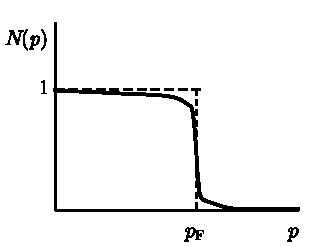
\includegraphics[width=5.2cm]{fig1.pdf}\\[0.3em]{\small 图 1}
\end{minipage}\par\nopagebreak

分布函数 $N(\bm p)$ 可以通过格林函数用(7.23)式的积分表达出来（图1）. 由于函数 $g(\omega,\bm p)$ 是有限的，可以预见它的积分之差当 $q\to0$ 时将趋于零. 因此，只研究(10.2)式中各极点项积分之差也就足够了. 由于在积分时分母中 i0 项只在极点附近才是重要的，所以§9中已指出，可将 $\mathrm{sign}\,\bm\omega$ 换写成 $\mathrm{sign}(p-p_{\mathrm F})$. 于是我们有
\begin{equation*}
N(p_{\mathrm F}-q)-N(p_{\mathrm F}+q)=-\mathrm{i}\int_{-\infty}^{\infty}\bigg\{\frac{Z}{\omega+v_{\mathrm F}q-\mathrm{i}0}-\frac{Z}{\omega-v_{\mathrm F}q+\mathrm{i}0}\bigg\}\frac{\mathrm{d}\omega}{2\pi}
\end{equation*}
（由于此两项差的积分是收敛的，所以 $t=-0$ 的因子 $\mathrm{e}^{-\mathrm{i}\omega t}$ 可以从积分中略去）. 现在用无限远的半圆周（随便哪个半平面内的半圆周）来封闭积分路线，我们求得整个积分等于 $Z$ 并与 $q$ 无关. 因此有
\begin{equation}
N(p_{\mathrm F}-0)-N(p_{\mathrm F}+0)=Z
\end{equation}
［А.\,Б.\,Мигдал, 1957］.

上面我们已经指出，$Z>0$. 由于 $N(\bm p)\leqslant1$，所以根据(10.3)式可得
\begin{equation}
0<Z\leqslant1
\end{equation}
（并且仅在理想气体的极限情况下才能达到 $Z=1$ 的值）.

因此，$T=0$ 时费米液体中粒子按动量的分布，如在气体中的情况一样在费米球面处有跃变，并且从球内向球外方向减小. 但是，与气体情况不同的是，跃变的值是小于1的，甚至当 $p>p_{\mathrm F}$ 时，函数 $N(\bm p)$ 仍不等于零，如图1中的实线曲线所示（虚线相应于气体）.

\section{由格林函数计算热力学量}

知道了系统的格林函数，就足以描写它的热力学性质. 当 $T=0$ 时，这些性质可以用系统的能量（与基态能量 $E_0$ 相同）与密度 $N/V$ 的关系表达出来.

解方程(8.16)之后便确定了准粒子的色散律 $\bm\varepsilon(\bm p)$，这种关系可以利用等式
\begin{equation}
\bm\varepsilon(p_{\mathrm F})=\bm\mu
\end{equation}
求出. 由于 $p_{\mathrm F}$ 与 $N/V$ 的关系是已知的，根据(1.1)，
\begin{equation}
p_{\mathrm F}=(3\pi^2)^{1/3}(N/V)^{1/3},
\end{equation}
等式(11.1)决定了函数 $\bm\mu(N/V)$［尽管这是隐函数形式，因为一般说来色散律 $\bm\varepsilon(\bm p)$ 含有参量 $\bm\mu$］. 当 $T=0$（因此 $S=0$）时，化学势 $\bm\mu=(\partial E_0/\partial N)_V$；将上述等式取积分，我们可得待求的能量
\begin{equation}
E_0=\int_0^N\bm\mu\Big(\frac{N}{V}\Big)\mathrm{d}N
\end{equation}
（当 $N=0$ 时，自然 $E_0=0$）.

描写 $T=0$ 时热力学性质的另一种方法是计算热力学势 $\Omega$. 根据普遍的定义（见第五卷§24），热力学势 $\Omega=E-TS-\bm\mu N=-PV$，它的微分 $\mathrm{d}\Omega=-S\mathrm{d}T-N\mathrm{d}\bm\mu$；当 $T=\bm 0$ 时，也有 $S=0$，于是这两个表达式归结为
\begin{equation}
\Omega=E-\bm\mu N,
\end{equation}
\begin{equation}
\mathrm{d}\Omega=-N\mathrm{d}\bm\mu.
\end{equation}

我们记得，依据热力学势 $\Omega$ 的意义，它描写体积 $V$ 为常数时系统的性质.

通过格林函数表示 $\Omega$ 的一种简易方法，是运用 $N/V$ 与 $G$ 的(7.24)式关系. 将(7.24)式的 $N$ 代入(11.5)式，并对 $\mathrm{d}\bm\mu$ 进行积分（当 $V=$ 常数时），因为当 $\bm\mu=0$ 时仍有 $\Omega=0$，我们得到
\begin{equation}
\Omega(\bm\mu)=2\mathrm{i}V\int_0^{\bm\mu}\mathrm{d}\bm\mu\cdot\lim_{t\to-0}\int G(\omega,\bm p)\,\mathrm{e}^{-\mathrm{i}\omega t}\frac{\mathrm{d}^3p\,\mathrm{d}\omega}{(2\pi)^4}.
\end{equation}

\section{相互作用绘景中的\texorpdfstring{$\psi$}{ψ}算符}

相互作用粒子系统的格林函数，当然不能以一般的形式计算出来. 但是有一种数学方法（类似于量子场论中的图技术）可以按粒子相互作用能的幂级数形式将它算出来. 并且级数的每一项都通过自由粒子系统的格林函数和相互作用算符表达出来.

除了算符的海森伯绘景之外，我们还引入另一种绘景，在这种绘景里算符与时间的关系不决定于系统的真实哈密顿量
\begin{equation*}
\hat H'=\hat H'^{(0)}+\hat V=\hat H^{(0)}-\bm\mu\hat N+\hat V
\end{equation*}
（$\hat V$ 是相互作用算符），而决定于自由粒子的哈密顿量 $\hat H'^{(0)}$：
\begin{equation}
\hat\Psi_0(t,\bm r)=\exp\big(\mathrm{i}\hat H'^{(0)}t\big)\hat\psi(\bm r)\exp\big(-\mathrm{i}\hat H'^{(0)}t\big).
\end{equation}

我们将用下标0来标记该绘景（即所谓相互作用绘景）中的算符和波函数，以示区别. 如将格林函数通过算符 $\hat\Psi_0$（代替海森伯算符 $\hat\Psi$）表达出来，我们便做到了用 $G^0$ 和 $\hat V$ 表达 $G$ 这一目的的第一步.

在这一节里，我们用记号 $\varPhi$（或 $\varphi$）代表“占有数空间”中的波函数（以区别于坐标波函数 $\hat\Psi$ 或 $\hat\psi$）；二次量子化算符就作用在这些波函数上. 令 $\varphi$ 为薛定谔绘景中的波函数，它与时间的关系决定于波动方程
\begin{equation}
\mathrm{i}\,\frac{\partial\varphi}{\partial t}=\big(\hat H'^{(0)}+\hat V\big)\varphi.
\end{equation}

在海森伯绘景中，所有时间关系都转到算符上，而系统的波函数则与时间无关：$\varPhi=$ 常数. 在相互作用绘景中，波函数 $\varPhi_0$ 依赖于时间，但这种依赖关系只与系统中粒子的相互作用有关，并决定于方程
\begin{equation}
\mathrm{i}\,\frac{\partial}{\partial t}\varPhi_0(t)=\hat V_0(t)\varPhi_0(t)
\end{equation}
式中
\begin{equation}
\hat V_0=\exp\big(\mathrm{i}\hat H'^{(0)}t\big)\hat V\exp\big(-\mathrm{i}\hat H'^{(0)}t\big).
\end{equation}

它是这个绘景中的相互作用算符［简单地把 $\hat\Psi$ 换成 $\hat\Psi_0$ 便使(7.6—7.7)形式的算符过渡到这个绘景中］. 注意，只要根据(12.1)式变换算符，即相应于按照
\begin{equation}
\varPhi_0=\exp\big(\mathrm{i}\hat H'^{(0)}t\big)\varphi,
\end{equation}
变换波函数（见第三卷§12），便不难得到方程(12.3). ［考虑到(12.2)式，并对上式取微商则得方程(12.3)\footnote{方程(12.3)与第四卷的方程(73.5)是相同的，在下面求解方程的过程中还将重复第四卷 §73 的叙述.}］.

基于方程(12.3)，函数 $\varPhi_0(t)$ 在两个无限接近时刻的值由下列等式相联系：
\begin{equation*}
\varPhi_0(t+\delta t)=\big[1-\mathrm{i}\delta t\cdot\hat V_0(t)\big]\varPhi_0(t)=\exp\big\{-\mathrm{i}\delta t\cdot\hat V_0(t)\big\}\varPhi_0(t).
\end{equation*}
相应地，$\varPhi_0$ 在任一时刻 $t$ 的值可以通过某一初始时刻 $t_0$ ($t_0<t$) 的值表达成
\begin{equation}
\varPhi_0(t)=\hat S(t,t_0)\varPhi_0(t_0),
\end{equation}
式中
\begin{equation}
\hat S(t,t_0)=\prod_{t_i=t_0}^{t}\exp\{-\mathrm{i}\delta t\cdot\hat V_0(t_i)\}.
\end{equation}

并且，此乘积中诸因子显然是按时间 $t_i$ 增长的次序从右向左排列的；对 $t_0$ 和 $t$ 之间一切无限小区间 $\delta t$ 的乘积是有极限的. 如果 $V_0(t)$ 是普通的函数，则这个极限将简单地归结为
\begin{equation*}
\exp\Big\{-\mathrm{i}\int_{t_0}^{t}V_0(t)\,\mathrm{d}t\Big\}.
\end{equation*}

但这种归结要根据不同时刻因子的可对易性，后者指的是：由(12.7)式中的乘积过渡到指数中的求和. 对于算符 $\hat V_0(t)$，则没有这种对易性，因而不可能归结为通常的积分. 代替积分式可以把(12.7)式写成符号形式：
\begin{equation}
\hat S(t,t_0)=T\exp\Big\{-\mathrm{i}\int_{t_0}^{t}\hat V_0(t)\,\mathrm{d}t\Big\}.
\end{equation}

这里 $T$ 是与(12.7)式相同顺序中因子的编时排列符号，即由右向左表示时间增长的顺序.

算符 $\hat S$ 是幺正的（$\hat S^{-1}=\hat S^{+}$），并具有明显的性质：
\begin{equation}
\begin{aligned}
&\hat S(t_3,t_2)\hat S(t_2,t_1)=\hat S(t_3,t_1),\\
&\hat S^{-1}(t_2,t_1)\hat S^{-1}(t_3,t_2)=\hat S^{-1}(t_3,t_1).
\end{aligned}
\end{equation}

为了简化以下的讨论，我们作一个纯形式上的假定（不反映在最后结果中），即相互作用 $\hat V_0(t)$ 从时刻 $t=-\infty$ 到有限的时间浸渐地“引入”，并在 $t=+\infty$ 时又浸渐地“除去”. 这样，当 $t\to-\infty$ 到引入相互作用之前，波函数 $\varPhi_0(t)$ 与海森伯波函数 $\varPhi$ 是一致的. 在(12.6)式中，令 $t_0=-\infty$，可得
\begin{equation}
\varPhi_0(t)=\hat S(t,-\infty)\varPhi.
\end{equation}

因此，建立了两个绘景波函数之间的关系，我们也就确定了算符的变换规律，其中包括 $\psi$ 算符的变换规律：
\begin{equation}
\hat\Psi=\hat S^{-1}(t,-\infty)\hat\Psi_0\hat S(t,-\infty).
\end{equation}

由于 $\hat S$ 的幺正性，所以算符 $\hat\Psi^{+}$ 也按同样规律变换.

现在我们把格林函数用相互作用绘景的 $\psi$ 算符表达出来\footnote{这个推导重复了第四卷 §103 中的讨论.}. 令 $t_1>t_2$，于是
\begin{equation*}
\begin{aligned}
G_{\alpha\beta}(X_1,X_2)&=-\mathrm{i}\langle\hat\Psi_\alpha(t_1)\hat\Psi^{+}_\beta(t_2)\rangle=\\
&=-\mathrm{i}\big\langle\hat S^{-1}(t_1,-\infty)\hat\Psi_{0\alpha}(t_1)\hat S(t_1,-\infty)\hat S^{-1}(t_2,-\infty)\times\\
&\quad\times\hat\Psi^{+}_{0\beta}(t_2)\hat S(t_2,-\infty)\big\rangle.
\end{aligned}
\end{equation*}

根据(12.9)式，我们有
\begin{equation*}
\begin{aligned}
\hat S(t_1,-\infty)\hat S^{-1}(t_2,-\infty)&=\hat S(t_1,t_2)\hat S(t_2,-\infty)\hat S^{-1}(t_2,-\infty)=\\
&=\hat S(t_1,t_2),\\
\hat S^{-1}(t_1,-\infty)&=\hat S^{-1}(t_1,-\infty)\hat S^{-1}(\infty,t_1)\hat S(\infty,t_1)=\\
&=\hat S^{-1}(\infty,-\infty)\hat S(\infty,t_1).
\end{aligned}
\end{equation*}

将它们代入前一个表达式，则得
\begin{equation*}
G_{\alpha\beta}(X_1,X_2)=-\mathrm{i}\big\langle\hat S^{-1}(\infty,-\infty)\hat S(\infty,t_1)\hat\Psi_{0\alpha}(t_1)\hat S(t_1,t_2)\hat\Psi^{+}_{0\beta}(t_2)\hat S(t_2,-\infty)\big\rangle.
\end{equation*}

把算符 $\hat S$ 理解为(12.7)式的乘积时，我们看到，平均值表达式中从第二个因子起的所有因子都是按由 $t=-\infty$ 到 $t=\infty$ 的编时顺序从右向左排列的. 因此可以写成
\begin{equation}
G_{\alpha\beta}(X_1,X_2)=-\mathrm{i}\langle\hat S^{-1}T[\hat\Psi_{0\alpha}(t_1)\hat\Psi^{+}_{0\beta}(t_2)\hat S]\rangle.
\end{equation}
式中的记号
\begin{equation}
\hat S\equiv\hat S(\infty,-\infty)=T\exp\Big\{-\mathrm{i}\int_{-\infty}^{\infty}\hat V_0(t)\,\mathrm{d}t\Big\}.
\end{equation}

当 $t_1<t_2$ 时，计算方法与上述算法的区别只在于记号的不同，(12.12—12.13)式的最后结果，对任意的 $t_1,t_2$ 都是正确的.

以上所作的变换与系统在什么状态上进行平均是无关的. 但是，如果对基态进行平均［如(12.12)］，变换还可以继续推广. 对此我们指出，浸渐引入或浸渐除去相互作用，如同任何浸渐微扰一样都不能引起量子系统发生能量改变的跃迁（见第三卷§41）. 因此，处于非简并态（基态也是这样的态）的系统，仍旧留在原来状态. 换言之，算符 $\hat S$ 作用在波函数 $\varPhi=\varPhi_0(-\infty)$ 上，归结为对 $\varPhi$ 乘以（对状态无关紧要的）一个相因子——算符 $\hat S$ 在基态的平均值：$\hat S\varPhi=\langle\hat S\rangle\varPhi$. 恰好 $\varPhi^{*}\hat S^{-1}=\langle S\rangle\varPhi^{*}$ 也是如此. 这样，我们最终得到了通过相互作用绘景的算符所表达的如下格林函数公式\footnote{应当指出，(12.14)式中关于符号有一个约定：虽然符号 $T$ 在公式中出现两次（一是以显形式，二是包含在 $\hat S$ 的定义中），但实际上乘积中所有因子都应按统一的编时顺序排列.}：
\begin{equation}
\mathrm{i}G_{\alpha\beta}(X_1,X_2)=\frac{1}{\langle\hat S\rangle}\big\langle T[\hat\Psi_{0\alpha}(X_1)\hat\Psi^{+}_{0\beta}(X_2)\hat S]\big\rangle.
\end{equation}

按这个绘景的意义，(12.14)式是对自由粒子系统的基态进行平均的. 事实上，算符 $\hat\Psi_0$ 的性质与无相互作用时海森伯算符 $\hat\Psi$ 的性质相同. 而海森伯波函数 $\varPhi$ 与时间无关，因此它与 $t=-\infty$（这时不存在相互作用）时的自身值相合. 所以，例如
\begin{equation}
\langle T\hat\Psi_{0\alpha}(X_1)\hat\Psi^{+}_{0\beta}(X_2)\rangle=\mathrm{i}G^{(0)}_{\alpha\beta}(X_1,X_2)
\end{equation}
就是无相互作用粒子系统的格林函数.

\section{费米系统的图技术}

(12.14)型的符号表达式的意义，在于有可能容易写出按 $\hat V$ 的幂展开的数列之各项. 例如
\begin{equation}
\begin{aligned}
&\big\langle T\hat\Psi_{0\alpha}(X)\hat\Psi^{+}_{0\beta}(X')\hat S\big\rangle=\\
&\qquad=\sum_{n=0}^{\infty}\frac{(-\mathrm{i})^n}{n!}\int_{-\infty}^{\infty}\mathrm{d}t_1\cdots\int_{-\infty}^{\infty}\mathrm{d}t_n\,\big\langle T\hat\Psi_{0\alpha}(X)\hat\Psi^{+}_{0\beta}(X')\hat V_0(t_1)\cdots\hat V_0(t_n)\big\rangle.
\end{aligned}
\end{equation}
而 $\langle\hat S\rangle$ 的表达式不同于上式的地方，仅在于 $T$ 乘积记号后没有因子 $\hat\Psi_{0\alpha}\hat\Psi^{+}_{0\beta}$. 我们已经指出过，相互作用绘景中的算符 $\hat V_0(t)$ 是将(7.7)式中所有的 $\hat\Psi$ 换成 $\hat\Psi_0$ 而得出的. 因此，计算(13.1)展开式数列的各个项，归结为计算自由粒子不同数量的 $\psi$ 算符的 $T$ 乘积对基态的平均值.

这些计算，在很大程度上是借助图技术规则而自动进行的，不过这些规则与被研究的物理系统的性质有重要关系. 这一节所叙述的图技术是关于非超流费米系统的. 其中假定相互作用是粒子成对式的，并与自旋无关. 相应的相互作用算符为：
\begin{equation}
\hat V_0(t)=\frac{1}{2}\int\hat\Psi^{+}_{0\gamma}(t,\bm r_1)\hat\Psi^{+}_{0\delta}(t,\bm r_2)U(\bm r_1-\bm r_2)\hat\Psi_{0\delta}(t,\bm r_2)\hat\Psi_{0\gamma}(t,\bm r_1)\,\mathrm{d}^3x_1\,\mathrm{d}^3x_2.
\end{equation}
式中 $U(\bm r_1-\bm r_2)$ 为两个粒子的相互作用能［我们省略了 $\hat V$ 和 $\hat U$ 的上标(2)］.

借助维克定理可以算出 $\psi$ 算符乘积的平均值，该定理的内容是\footnote{为了不中断叙述，我们把这个定理的证明放在本节之末.}：

任意数目成对算符 $\hat\Psi$ 跟 $\hat\Psi^{+}$ 乘积的平均值，等于这些算符一切可能的成对平均值（收缩）乘积之和. 每一对算符的先后次序与原始乘积中的一致. 求和式中每一项的符号决定于因子 $(-1)^P$，这里 $P$ 是算符的置换次数，进行这些置换是使所有被平均的算符都并排在邻接的位置上.

只有包含一个算符 $\hat\Psi$ 和一个算符 $\hat\Psi^{+}$ 的收缩才不为零，因为在对角矩阵元中，一切被算符 $\hat\Psi$ 消灭的粒子应重新被算符 $\hat\Psi^{+}$ 产生. 由此可见，在一些 $\psi$ 算符的乘积中如果只包含相同数目的算符 $\hat\Psi$ 和 $\hat\Psi^{+}$，该乘积的平均值才能不等于零.

将维克定理应用于 $T$ 乘积的平均值，则该平均值就能通过成对的 $T$ 乘积的平均值［根据(12.15)式，即通过自由粒子格林函数］表达出来. 下面计算相互作用粒子系统格林函数的一级修正. 我们预先指出，按照维克定理将公式(12.14)分子中的表达式展开时，例如会出现如下形式的一些项：
\begin{equation}
\big\langle T\hat\Psi_{0\alpha}(X_1)\hat\Psi^{+}_{0\beta}(X_2)\big\rangle\langle\hat S\rangle=\mathrm{i}G^{(0)}_{\alpha\beta}(X_1,X_2)\langle\hat S\rangle
\end{equation}
在这些项中，一对（相对于 $\hat S$）的“外部”$\psi$ 算符之间是收缩的，而 $\langle\hat S\rangle$ 的表达式（它的展开式的每一项中）只含“内部”算符之间的收缩. 因子 $\langle\hat S\rangle$ 可被(12.14)式中的分母完全约去，因此所有这些项简便地给出了“无微扰的”格林函数 $\mathrm{i}G^{(0)}_{\alpha\beta}$.

在(13.1)式中保留展开式的前两项，将(13.2)式代入并变换变量，我们得到
\begin{equation*}
\mathrm{i}G_{\alpha\beta}(X_1,X_2)\approx\mathrm{i}G^{(0)}_{\alpha\beta}+\mathrm{i}G^{(1)}_{\alpha\beta}.
\end{equation*}
式中
\begin{equation*}
\begin{aligned}
\mathrm{i}G^{(1)}_{\alpha\beta}&=-\frac{\mathrm{i}}{2}\big\langle T\hat\Psi_{0\alpha}(X_1)\hat\Psi^{+}_{0\beta}(X_2)\times\\
&\quad\times\int_{-\infty}^{\infty}\mathrm{d}t\,\mathrm{d}^3x_3\,\mathrm{d}^3x_4\,\hat\Psi^{+}_{0\gamma}(t,\bm r_3)\hat\Psi^{+}_{0\delta}(t,\bm r_4)U(\bm r_3-\bm r_4)\hat\Psi_{0\delta}(t,\bm r_4)\hat\Psi_{0\gamma}(t,\bm r_3)\big\rangle.
\end{aligned}
\end{equation*}
为了把公式写得更紧凑一些，我们引入记号
\begin{equation}
U(X_1-X_2)=U(\bm r_1-\bm r_2)\,\delta(t_1-t_2),
\end{equation}
于是\footnote{此后，为了简化特别烦琐的表达式的书写，我们约定略去 $\hat\Psi_{0}$ 的下标，而用数字下标 $1,2,\cdots$，来标记宗量数值 $X$ 和自旋下标的总体：
\begin{gather*}
\hat\Psi_{1}\equiv\hat\Psi_{\alpha}(X_{1}),\qquad
\hat\Psi_{2}\equiv\hat\Psi_{\beta}(X_{2}),\cdots\\
G_{12}\equiv G_{\alpha\beta}(X_{1},X_{2}),\qquad
U_{12}\equiv U(X_{1}-X_{2}).
\end{gather*}}
\begin{equation*}
\mathrm{i}G^{(1)}_{12}=-\frac{\mathrm{i}}{2}\int\big\langle T\hat\Psi_1\hat\Psi^{+}_2\hat\Psi^{+}_3\hat\Psi^{+}_4\hat\Psi_4\hat\Psi_3\big\rangle U_{34}\,\mathrm{d}^4X_3\,\mathrm{d}^4X_4,
\end{equation*}
式中 $\mathrm{d}^4X=\mathrm{d}t\,\mathrm{d}^3x$.

为了按照维克定理求平均，我们分别写出算符，并画出所有需要收缩的方式：
\begin{equation*}
\begin{aligned}
\langle\Psi_1\Psi^{+}_2\Psi^{+}_3\Psi^{+}_4\Psi_4\Psi_3\rangle\to{}\;&
\overset{\frown}{\Psi_1}\underset{\smile}{\Psi^{+}_2}\overset{\frown}{\Psi^{+}_3}\,\overset{\smile}{\Psi^{+}_4}\underset{\smile}{\Psi_4}\overset{\smile}{\Psi_3}+{}\\
&+\overset{\frown}{\Psi_1}\overset{\smile}{\Psi^{+}_2}\underset{\smile}{\Psi^{+}_3}\,\overset{\frown}{\Psi^{+}_4}\underset{\smile}{\Psi_4}\overset{\smile}{\Psi_3}+\\
&+\overset{\frown}{\Psi_1}\overset{\smile}{\Psi^{+}_2}\overset{\frown}{\Psi^{+}_3}\,\underset{\smile}{\Psi^{+}_4}\underset{\smile}{\Psi_4}\overset{\smile}{\Psi_3}+\\
&+\overset{\frown}{\Psi_1}\underset{\smile}{\Psi^{+}_2}\overset{\smile}{\Psi^{+}_3}\,\overset{\frown}{\Psi^{+}_4}\underset{\smile}{\Psi_4}\overset{\smile}{\Psi_3}.
\end{aligned}
\end{equation*}
（同一标记的两端点为互相收缩的一对.）根据上边所述，含 $\overset{\frown}{\Psi_1\Psi^{+}_2}$ 收缩的各项已被略去. 成对收缩的（用弧线联结的）算符应置换到彼此邻接的位置. 例如，所写出的第一项表示下列乘积：
\begin{equation*}
\langle T\hat\Psi_1\hat\Psi^{+}_3\rangle\langle T\hat\Psi^{+}_2\hat\Psi_4\rangle\langle T\hat\Psi^{+}_4\hat\Psi_3\rangle,
\end{equation*}
而最后一项表示
\begin{equation*}
-\langle T\hat\Psi_1\hat\Psi^{+}_4\rangle\langle T\hat\Psi^{+}_2\hat\Psi_4\rangle\langle T\hat\Psi^{+}_3\hat\Psi_3\rangle.
\end{equation*}

不同宗量 $\psi$ 算符的收缩，可根据下列式子代换：
\begin{equation*}
\overset{\frown}{\Psi_1\Psi^{+}_3}\equiv\langle T\hat\Psi_1\hat\Psi^{+}_3\rangle=\mathrm{i}G^{0}_{13},\quad \overset{\frown}{\Psi^{+}_2\Psi_4}=-\mathrm{i}G^{0}_{24},\ \text{等等.}
\end{equation*}

相同宗量 $\psi$ 算符的收缩，乃是理想气体中粒子数的空间密度（用 $n^{(0)}$ 标记），该密度可理解为化学势的函数\footnote{这些收缩总是出自于同一个相互作用算符 $\hat V$ 中的 $\psi$ 算符. 因此，在这些项中 $\hat\Psi^{+}$ 总是排在 $\hat\Psi$ 的左边.}：
\begin{equation}
\langle\hat\Psi^{+}\hat\Psi\rangle=n^{(0)}(\bm\mu)=\frac{(2m\bm\mu)^{3/2}}{3\pi^2},
\end{equation}

所以可得
\begin{equation*}
\begin{aligned}
\mathrm{i}G^{(1)}_{12}=\frac{1}{2}\int\mathrm{d}^4X_3\,\mathrm{d}^4X_4\cdot U_{34}\big[&-G^{(0)}_{13}G^{(0)}_{34}G^{(0)}_{42}-G^{(0)}_{14}G^{(0)}_{43}G^{(0)}_{32}+\\
&+\mathrm{i}n^{(0)}G^{(0)}_{13}G^{(0)}_{32}+\mathrm{i}n^{(0)}G^{(0)}_{14}G^{(0)}_{42}\big],
\end{aligned}
\end{equation*}
这四项两两相等，它们的区别仅在于积分变量 $X_3$ 和 $X_4$ 的记号不同. 因之因子 $1/2$ 消失，所以格林函数的一级修正只包含两项：
\begin{equation}
\mathrm{i}G^{(1)}_{12}=\int U_{34}\big[\mathrm{i}n^{(0)}G^{(0)}_{14}G^{(0)}_{42}-G^{(0)}_{13}G^{(0)}_{34}G^{(0)}_{42}\big]\mathrm{d}^4X_3\,\mathrm{d}^4X_4.
\end{equation}

借助如下的费曼图可以用图解法方便地表示出这些项的结构：
\begin{equation}
\raisebox{-0.35\height}{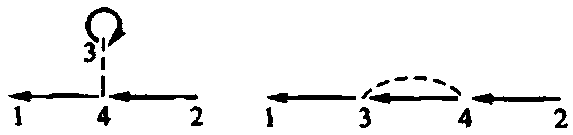
\includegraphics[width=9.6cm]{feyn13-07.png}}
\end{equation}

在这些图中，实线 $4\leftarrow2$ 表示收缩 $\overset{\frown}{\Psi_4\Psi^{+}_2}$（即函数 $\mathrm{i}G^{(0)}_{42}$）；数字表示变量 $X_4$ 和 $X_2$ 的号码，收缩的算符与这些变量有关，而箭头的方向与收缩中从 $\hat\Psi^{+}$ 到 $\hat\Psi$ 的方向一致. 依赖于相同变量的两个算符的收缩 $\overset{\frown}{\Psi^{+}\Psi}$（即粒子数密度 $n^{(0)}$），相应地用“自身封闭的”实线圈图表示. 虚线 $3\text{---}4$ 表示因子 $U_{34}$. 图形的各内点（线的交点），是指按它们标记的所有变量取积分. 图形“外端点”标记的变量（$X_1$ 和 $X_2$）仍是自由的.

例如，由(13.3)式得出的各一级项，将用被分解为两个独立部分——直线段（$\mathrm{i}G^{(0)}_{\alpha\beta}$）和实线封闭圈图表示：
\begin{equation*}
\raisebox{-0.35\height}{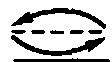
\includegraphics[height=0.75cm]{feyn13-loop.png}}
\end{equation*}

仔细考虑算符的收缩方式和相应的图形结构，就能了解普遍规则的来历，因为在微扰论的一切级中，(12.14)式中因子 $\langle S\rangle^{-1}$ 的作用归结为：只需考虑有两个外线的“相连”图形，这些图形不包含“不相连的”无外线的圈图. 后者与图形的其它部分均不相连（既无实线相连也无虚线相连）（对照量子电动力学中类似的情况——第四卷§100）.

在(13.6)式中消去系数1/2反映了一个通则：无须考虑出现在(13.1)展开式中各 $n$ 级项的因子 $1/n!$，也无须考虑来自(13.2)式中系数1/2的因子 $2^{-n}$. 的确，$n$ 级图形每个都包含着 $n$ 条虚线 $i\text{---}k$. 消去因子 $1/n!$ 是由于叠加了不同的项，这些项是沿所有 $n$ 条虚线置换一对指标 $i,k$ 而得到的. 消去因子 $2^{-n}$ 是由于在每一条线两端点之间都有 $i,k$ 的置换.

现在我们来说明在动量表象（不是坐标表象）中计算格林函数时既定的图技术规则，这在物理学最为有用.

借助傅里叶展开式(7.21—7.22)可以实现向动量表象的过渡，我们将展开式写成“4维”形式\footnote{为了叙述和表达的方便，我们利用了 4 维的术语，再强调一次，这里它与相对论不变性无任何关系！}
\begin{equation}
G(X)=\int G(P)\,\mathrm{e}^{-\mathrm{i}PX}\frac{\mathrm{d}^4P}{(2\pi)^4},\qquad G(P)=\int G(X)\,\mathrm{e}^{\mathrm{i}PX}\mathrm{d}^4X,
\end{equation}
式中“4维动量”$P=(\omega,\bm p)$，$PX=\omega t-\bm p\cdot\bm r$. 用类似的方法同样可以把相互作用势展开成：
\begin{equation}
U(X)=\delta(t)U(\bm r)=\int U(Q)\,\mathrm{e}^{-\mathrm{i}QX}\frac{\mathrm{d}^4Q}{(2\pi)^4}
\end{equation}
其中 $Q=(q_0,\bm q)$；而且 $U(Q)$ 与三维展开式的分量一致：
\begin{equation}
U(Q)\equiv U(\bm q)=\int U(\bm r)\,\mathrm{e}^{-\mathrm{i}\bm q\cdot\bm r}\,\mathrm{d}^3x.
\end{equation}
由于 $U(\bm r)$ 是偶函数，显然 $U(-\bm q)=U(\bm q)$.

我们对一级修正 $G^{(1)}_{12}\equiv G^{(1)}_{\alpha\beta}(X_1-X_2)$ 进行这种展开. 为此，给等式(13.6)乘以 $\exp[\mathrm{i}P(X_1-X_2)]$ 并将该式对 $\mathrm{d}^4(X_1-X_2)$ 积分.

在第一项内写出
\begin{equation*}
\mathrm{e}^{\mathrm{i}P(X_1-X_2)}=\mathrm{e}^{\mathrm{i}P(X_1-X_3)}\,\mathrm{e}^{\mathrm{i}P(X_3-X_2)}.
\end{equation*}
变换积分变量，于是得到
\begin{equation*}
\begin{aligned}
&\mathrm{i}n^{(0)}\int G^{(0)}_{\alpha\gamma}(X_1-X_3)\,\mathrm{e}^{\mathrm{i}P(X_1-X_3)}\,\mathrm{d}^4(X_1-X_3)\times\\
&\qquad\times\int G^{(0)}_{\gamma\beta}(X_3-X_2)\,\mathrm{e}^{\mathrm{i}P(X_3-X_2)}\,\mathrm{d}^4(X_3-X_2)\int U(X_3-X_4)\,\mathrm{d}^4(X_3-X_4).
\end{aligned}
\end{equation*}
前两个积分给出 $G^{(0)}_{\alpha\gamma}(P)G^{(0)}_{\gamma\beta}(P)$，第三积分等于 $U(0)=\int U(\bm r)\,\mathrm{d}^3x$，即 $U(\bm q)$ 在 $\bm q=0$ 的值.

采用类似的方法，在第二项内写出
\begin{equation*}
\mathrm{e}^{\mathrm{i}P(X_1-X_2)}=\mathrm{e}^{\mathrm{i}P(X_1-X_3)}\,\mathrm{e}^{\mathrm{i}P(X_3-X_4)}\,\mathrm{e}^{\mathrm{i}P(X_4-X_2)}.
\end{equation*}
转为对 $X_1-X_3,\ X_3-X_4,\ X_4-X_2$ 的积分之后，可得
\begin{equation*}
-G^{(0)}_{\alpha\gamma}(P)\int G^{(0)}_{\gamma\delta}(X)U(X)\,\mathrm{e}^{\mathrm{i}PX}\,\mathrm{d}^4X\cdot G^{(0)}_{\delta\beta}(P).
\end{equation*}

其余的积分，利用两个函数乘积的傅里叶分量公式，通过函数 $G^{(0)}_{\gamma\delta}$ 和 $U$ 的傅里叶分量表达出来\footnote{为了证明这个公式，需要将傅里叶展开形式的函数 $f(X)$ 和 $g(X)$ 代入该公式的左边：
\begin{equation*}
\int f(X)g(X)\,\mathrm{e}^{\mathrm{i}PX}\,\mathrm{d}^{4}X=\int f(P_{1})g(P_{2})\,\mathrm{e}^{\mathrm{i}(P-P_{1}-P_{2})X}\,\mathrm{d}^{4}X\,\frac{\mathrm{d}^{4}P_{1}\,\mathrm{d}^{4}P_{2}}{(2\pi)^{4}},
\end{equation*}
按下列公式对 $\mathrm{d}^{4}X$ 求积分：
\begin{equation*}
\int\mathrm{e}^{\mathrm{i}PX}\,\mathrm{d}^{4}X=(2\pi)^{4}\delta^{(4)}(P),
\end{equation*}
其中“4维”$\delta^{(4)}$ 函数定义为“4–矢量”$P$ 各分量的 $\delta$ 函数之积. 出现的因子 $\delta^{(4)}(P-P_{1}-P_{2})$ 被对 $\mathrm{d}^{4}P_{2}$ 的积分消掉，于是我们得出了(13.11)式的右边部分.}：
\begin{equation}
\int f(X)g(X)\,\mathrm{e}^{\mathrm{i}PX}\,\mathrm{d}^4X=\int f(P_1)g(P-P_1)\,\frac{\mathrm{d}^4P_1}{(2\pi)^4}.
\end{equation}

因此，对于动量表象中格林函数的一级修正，我们最后求得：
\begin{equation}
\begin{aligned}
\mathrm{i}G^{(1)}_{\alpha\beta}(P)&=\mathrm{i}n^{(0)}U(0)G^{(0)}_{\alpha\gamma}(P)G^{(0)}_{\gamma\beta}(P)-\\
&-\int G^{(0)}_{\alpha\gamma}(P)G^{(0)}_{\gamma\delta}(P_1)G^{(0)}_{\delta\beta}(P)U(\bm p-\bm p_1)\,\frac{\mathrm{d}^4P_1}{(2\pi)^4}.
\end{aligned}
\end{equation}

(13.12)式中右方每一项都对应于确定的费曼图，则表达式(13.12)可写成如下形式：
\begin{equation}
\mathrm{i}G^{(1)}_{\alpha\beta}(P)=
\raisebox{-0.45\height}{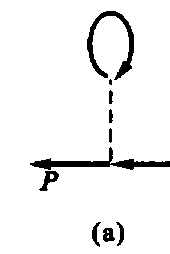
\includegraphics[height=1.9cm]{feyn13-13a.png}}-
\raisebox{-0.45\height}{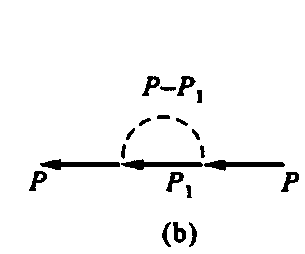
\includegraphics[height=1.9cm]{feyn13-13b.png}}
\end{equation}

各线的交点称作图形的顶点. 每个图形都有 $2n$ 个顶点，此处 $n$ 为微扰论的级. 在每个顶点上都汇聚两条实线和一条虚线. 每条实线在箭头指示的方向上描述“4维动量”$P$（并且，沿诸实线的每一连续序列，箭头的方向不变）. 每条虚线是用来标记4维动量 $Q$ 的，而且对于这些线，箭头可以约定取任何（任意）方向\footnote{4 维矢量 $Q=(q_{0},\bm q)$ 的“时间”分量，一般说来不等于零，但函数 $U(Q)$ 根据定义(13.10)与 $q_{0}$ 是无关的，虚线方向的约定，与偶函数 $U(-Q)=U(Q)$ 有关.}. 在图形的顶点上满足“4维动量守恒定律”：顶点的入射线的4维动量之和等于出射线的4维动量之和. 顶点也标出确定的自旋下标 $\alpha$. 每个图形都有两条外线（入射线和出射线），外线的4维动量是待求的格林函数 $G_{\alpha\beta}(P)$ 的宗量；出射和入射的外线同时也标记该函数的自旋下标 $\alpha$ 和 $\beta$. 图形其余的线称作内线.

相应于每个图形的各项，其解析表述法可按下列规则进行：

1）顶点 $\alpha$ 和 $\beta$ 之间的每条实线对应于因子 $\mathrm{i}G^{(0)}_{\alpha\beta}(P)$，每条虚线对应于因子 $-\mathrm{i}U(Q)$. 具有一个顶点的封闭圈图相当于因子 $n^{(0)}(\bm\mu)$.

2）在每个顶点上满足4维动量守恒定律. 将内线中其余不确定的4维动量对 $\mathrm{d}^4P/(2\pi)^4$ 进行积分. 在每个顶点上对一对自旋哑下标（从相邻接的 $G^{(0)}$ 因子中各取一个）进行求和.

3）$\mathrm{i}G_{\alpha\beta}$ 图的公共因子等于 $(-1)^L$，这里 $L$ 是图形中含有多于一个顶点的实线封闭圈图的数目.

最后一个规则的来由如下所述. 顶点数 $k>1$ 的封闭圈图，来源于如下形式的 $\psi$ 算符的收缩：
\begin{equation*}
\overset{\frown}{\Psi^{+}_1\Psi_1}\,\overset{\frown}{\Psi^{+}_2\Psi_2}\cdots\overset{\frown}{\Psi^{+}_k\Psi_k}
\end{equation*}
这里所有收缩分别等于 $\mathrm{i}G^{(0)}_{12},\cdots,\mathrm{i}G^{(0)}_{k-1,k}$，而最后一个收缩等于 $-\mathrm{i}G^{(0)}_{k1}$. 至于一个顶点的圈图，它们的正确符号在按规则1)引入 $n^{(0)}$ 时已考虑到了.

作为实例，我们汇总画出确定格林函数二级修正的图形：
\begin{equation}
\begin{tabular}{c@{\hspace{3em}}c@{\hspace{3em}}c}
\raisebox{-0.35\height}{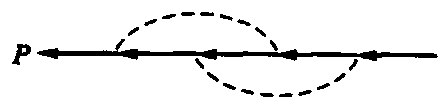
\includegraphics[height=0.85cm]{feyn13-14a.png}} &
\raisebox{-0.35\height}{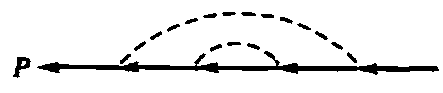
\includegraphics[height=0.75cm]{feyn13-14b.png}} & \\
(a) & (b) & \\[0.8em]
\raisebox{-0.35\height}{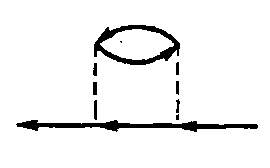
\includegraphics[height=1.15cm]{feyn13-14c.png}} &
\raisebox{-0.35\height}{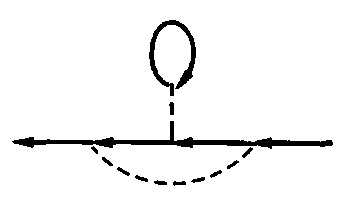
\includegraphics[height=1.25cm]{feyn13-14d.png}} &
\raisebox{-0.35\height}{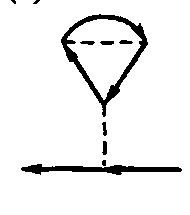
\includegraphics[height=1.3cm]{feyn13-14e.png}} \\
(c) & (d) & (e) \\[0.8em]
\raisebox{-0.35\height}{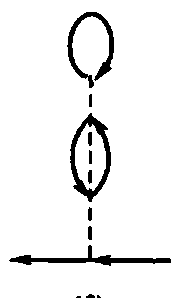
\includegraphics[height=1.5cm]{feyn13-14f.png}} &
\raisebox{-0.35\height}{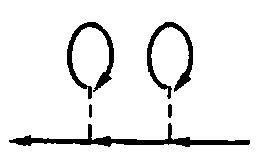
\includegraphics[height=1.05cm]{feyn13-14g.png}} &
\raisebox{-0.35\height}{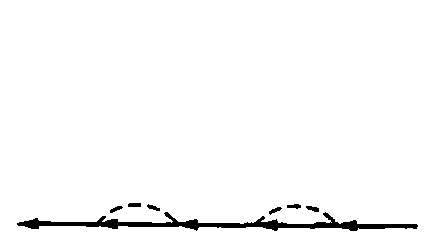
\includegraphics[height=1.25cm]{feyn13-14h.png}} \\
(f) & (g) & (h) \\[0.8em]
\raisebox{-0.35\height}{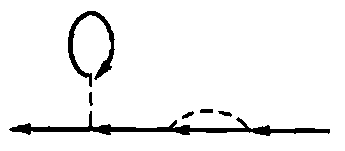
\includegraphics[height=0.95cm]{feyn13-14i.png}} &
\raisebox{-0.35\height}{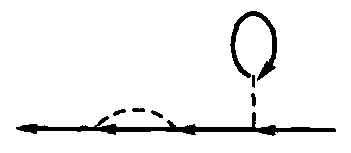
\includegraphics[height=0.95cm]{feyn13-14j.png}} & \\
(i) & (j) &
\end{tabular}
\end{equation}

最后，我们再来讨论维克定理，并给出它适于“宏观极限”（即当系统密度一定时 $V\to\infty$，或当系统密度一定时 $N\to\infty$）的证明，这在统计物理学的应用上恰恰是重要的.

例如，我们研究下列形式的四个 $\psi$ 算符乘积的平均值：
\begin{equation}
\big\langle\hat\Psi_{01}\hat\Psi_{02}\hat\Psi^{+}_{03}\hat\Psi^{+}_{04}\big\rangle=\frac{1}{V^2}\sum_{p_1\cdots p_4}\big\langle\hat a_{p_1}\hat a_{p_2}\hat a^{+}_{p_3}\hat a^{+}_{p_4}\big\rangle\exp(\cdots)
\end{equation}
［各 $\psi$ 算符表为(9.3)的形式；我们没写出显然的但又烦琐的指数函数标记］. 在这个求和式中，只有含动量值相同且数目相同的算符 $\hat a_{\bm p}$ 和 $\hat a^{+}_{\bm p}$ 的项才不为零. 其中有些项，动量成对地相等，如 $\bm p_1=\bm p_4$ 和 $\bm p_2=\bm p_3$. 这些项相应于成对的收缩：
\begin{equation*}
\underset{\smile}{\Psi_{01}\,\overset{\frown}{\Psi_{02}\Psi^{+}_{03}}\,\Psi^{+}_{04}}
\end{equation*}
并以如下形状的求和式来表达：
\begin{equation*}
\frac{1}{V^2}\sum_{p_1p_2}\big\langle\hat a_{p_1}\hat a^{+}_{p_1}\big\rangle\big\langle\hat a_{p_2}\hat a^{+}_{p_2}\big\rangle\exp(\cdots)
\end{equation*}
在极限 $V\to\infty$ 时，对 $\bm p_1$ 和 $\bm p_2$ 的求和可代之以对 $V^2\mathrm{d}^3p_1\,\mathrm{d}^3p_2/(2\pi)^6$ 的积分，这时消去了体积 $V$，而使表达式仍保持有限. 在(13.15)的求和式中，$\bm p_1=\bm p_2=\bm p_3=\bm p_4$ 的各项也不为零；这些项构成了下列形式之和：
\begin{equation*}
\frac{1}{V^2}\sum_{p}\big\langle\hat a_{p}\hat a_{p}\hat a^{+}_{p}\hat a^{+}_{p}\big\rangle\exp(\cdots)
\end{equation*}
但是，将求和变为积分之后还剩下一个因子 $1/V$，于是在极限 $V\to\infty$ 时表达式变成零.

显然，这个结果具有普遍性：在极限 $V\to\infty$ 时，$\psi$ 算符乘积的平均中只有成对收缩的结果才不变为零.

我们指出，在上述证明中实际上并没有真正对基态进行平均，因此这个证明在对系统的任何量子态求平均时仍是正确的\footnote{但是，如果对基态求平均，则维克定理就不限于在宏观极限时成立在统计学中相应的定理的证明与量子电动力学中（第四卷 §78）的证明是一致的. 它们之间唯一的区别是基态不同：在真空中没有粒子，而在理想气体中粒子占满半径为 $\bm p_{\mathrm F}$ 的费米球. 对于 $p>p_{\mathrm F}$ 的粒子的产生和湮没算符 $\hat a^{+}_{p},\hat a^{-}_{p}$ 来说，这种区别根本无关紧要，因此可以将证明逐字地移置到这里. 对于 $p<p_{\mathrm F}$ 粒子的算符，需要事先变换标记：$\hat a^{+}_{p}=b_{p},\hat a_{p}=\hat b^{+}_{p}$，也就是说由粒子变为空穴，而处于基态的空穴在费米球内是不存在的.}.
